\documentclass[preprint,12pt]{elsarticle}
\usepackage{amssymb}
\usepackage{amsmath}
\usepackage{graphicx}
\usepackage{booktabs}
\usepackage{multirow}
\usepackage{xcolor}
\usepackage{url}
\usepackage{algorithm}
\usepackage{algpseudocode}
\usepackage{hyperref}
\usepackage[capitalize,noabbrev]{cleveref}
\usepackage{tikz}
\usetikzlibrary{positioning,arrows.meta,fit}
\usepackage{amsthm}
\setlength{\emergencystretch}{2em}
\newtheorem{proposition}{Proposition}
\newtheorem{lemma}{Lemma}
% ---- Draft placeholders --------------------------------------------------
% While \drafttrue, placeholders render in colour. Set \draftfalse before
% submission: any leftover placeholder then stops compilation with an error.
\newif\ifdraft
\draftfalse
\DeclareRobustCommand{\TODO}[1]{\ifdraft{\color{orange}[TODO: #1]}\else\PackageError{draft}{Unresolved TODO: #1}{}\fi}
\DeclareRobustCommand{\RESULT}[1]{\ifdraft{\color{red}[RESULT: #1]}\else\PackageError{draft}{Missing experimental result: #1}{}\fi}
\DeclareRobustCommand{\CITE}[1]{\ifdraft{\color{blue}[CITE: #1]}\else\PackageError{draft}{Missing citation: #1}{}\fi}
\pdfstringdefDisableCommands{\def\TODO#1{TODO}\def\RESULT#1{RESULT}\def\CITE#1{CITE}}
% Allow compiling before any \cite{} is added to the draft:
\ifdraft\makeatletter\let\@noitemerr\relax\makeatother\fi

% ---- Notation (define symbols once; keep consistent with the notation table) ----
\newcommand{\ctx}{\mathbf{c}}          % context vector
\newcommand{\Ctx}{\mathcal{C}}         % context space
\newcommand{\Adv}{\mathcal{A}}         % adversary
\newcommand{\btheta}{\boldsymbol{\theta}}
\newcommand{\bx}{\boldsymbol{x}}
\newcommand{\bmu}{\boldsymbol{\mu}}
\newcommand{\bSigma}{\boldsymbol{\Sigma}}
\newcommand{\Aspace}{\mathcal{A}}
\newcommand{\Asafe}{\mathcal{A}_{\mathrm{safe}}}
\newcommand{\Iset}{\mathcal{I}_{\mathrm{safe}}}
\newcommand{\op}{\mathrm{op}}
\newcommand{\attack}{b^{\mathrm{atk}}}
\newcommand{\E}{\mathbb{E}}
\newcommand{\Prob}{\mathbb{P}}
\DeclareMathOperator*{\argmax}{arg\,max}
\newcommand{\ind}[1]{\mathbb{I}\!\left[#1\right]}


\begin{document}
\begin{frontmatter}
\title{Fail-Safe Context-Adaptive Access Control with Continuous Risk Belief Updates and Hard Safety Invariants for Cyber-Physical IoT}
\author[asu]{Mahmoud Aljawarneh}
\ead{ma_jawarneh@asu.edu.jo}
\affiliation[asu]{organization={Department of Cybersecurity and Cloud Computing, Applied Science Private University}}
\begin{abstract}
Context-adaptive access control (CAAC) lets IoT and cyber-physical deployments trade
authentication strength, inspection depth and session freshness against energy and
mission utility. When the context channel is spoofed, the same mechanism becomes an
attack surface: a coherent ``benign'' context can talk the policy below the posture
that the physical process requires. This paper separates the part of adaptation that
may be optimised from the part that may not. We formulate CAAC as a constrained
partially observable control problem over five latent threat states, with a forward
Bayesian belief, cross-modal consistency weights, and an admissible set defined by
unconditional invariants for actuation and safety-critical traffic. The controller
optimises expected utility only inside that set; if the set is empty it executes a
precomputed per-operation fail-safe action, and the enforcement point independently
re-checks the floor. A 24-node, 2{,}000-epoch, 10-seed simulation across seven attack
scenarios holds invariant violations at 0 per 1{,}000 decisions for every
invariant-enforcing policy, versus 393 for a static-low policy and 327 for
unconstrained risk adaptation. The full controller attains 0.120 mean
attack-scenario utility against 0.084 for static-high and 0.077 for threshold CAAC,
while denying 0.029 of safety-critical requests against 0.088. Residual exposure
remains and is reported: the full controller grants 0.177 of malicious requests
against 0.127 for static-high, concentrated in an explicitly out-of-model scenario
in which the node's trusted execution environment is subverted and the belief
collapses (Brier 0.437, poisoning AUROC 0.273). Within the stated threat model the
attested device anchor and cross-node dispersion survive poisoning, and the
guarantee is carried by the unconditional invariants rather than by detection. A
trace-derived calibration against IoT-23 sets the benign-to-malicious mean-log-rate
contrast to 1.69.

\end{abstract}
\begin{keyword}
context-adaptive access control \sep Internet of Things \sep cyber-physical systems \sep
colluding-minority robustness \sep Bayesian belief updating \sep safety invariants \sep
fail-safe enforcement
\end{keyword}
\end{frontmatter}

\section{Introduction}
\label{sec:intro}

Access control for the Internet of Things (IoT) is no longer a database
permission problem. A modern deployment authenticates battery-powered sensors,
issues commands to valves, locks and motors, and continuously re-evaluates who
may do what under changing load, link quality and physical state
\cite{ravidas2019access,qiu2020survey}. Context-adaptive access control (CAAC)
responds by making the security posture itself a function of context: a quiet
channel with a healthy battery may use a lighter handshake, while congestion or
anomalous telemetry triggers stronger authentication and deeper inspection
\cite{atlam2017overview,rath2017adaptive,genc2019context,arfaoui2019context}.
The promise is attractive because the alternative---a single high posture---is
expensive in energy, latency and false denials on constrained devices
\cite{elgendi2019protecting,elhajj2019survey}.

The same adaptability is an attack surface. An adversary who can influence the
context channel can make an unsafe posture look rational: spoof a low battery,
suppress anomaly evidence, or replay a benign-looking neighbourhood to drive the
policy below the level the physical process requires. Sensor spoofing and false
data injection are well documented in cyber-physical systems
\cite{barua2020special,li2019optimal,ye2020summation}, and denial-of-sleep
attacks show that forcing a device to over-react is equally effective
\cite{brownfield2005wireless,raymond2009effects}. Byzantine nodes can bias an
aggregate without controlling a majority \cite{lamport1982byzantine}, and a
periodic attacker can make an adaptive controller oscillate between postures
until it exhausts energy or its own hysteresis \cite{kephart2003vision,cheng2009software}.
Existing CAAC designs optimise expected utility against a point estimate of
risk and treat security strength as one more soft cost
\cite{lee2017situational,moura2017sotraace,hussainalnaji2022cab}. Under a
coherent spoof, the point estimate moves in the wrong direction, and because
nothing in the objective is non-negotiable, the optimiser follows it.

This paper starts from a different decomposition. \emph{Adaptation may choose
among safe actions, but it may not choose whether an action is safe.} We define
an admissible set $\Asafe(\op,\attack_t)$ from unconditional invariants---the
actuation envelope I1, the safety-traffic envelope I2, a belief-conditional
restriction I3, and per-operation failure semantics I4---and optimise mission
utility only inside that set. The invariants do not depend on the threat belief,
so a compromised or merely unlucky estimator cannot argue its way below them.
When the set would be empty, the enforcement point executes a precomputed safe
action: fail-closed for confidentiality and integrity operations, and
fail-safe-allow (authenticated emergency function only) where denial would
itself violate a physical safety requirement. This is runtime assurance in the
sense of Simplex and shield synthesis \cite{sha2001simplicity,wu2017safety,wu2019shield,mehmood2022black,cho2025timed},
but applied to an access-control action lattice rather than to a single
controller switch.

Inside the admissible set we keep uncertainty explicit. A forward hidden Markov
model maintains a belief over five latent threat states, and four context
modalities are fused with weights that fall when a modality's posterior drifts
from the device-telemetry anchor. The monitor therefore distinguishes ``the
plant is calm'' from ``the telemetry is lying'' as far as the evidence allows,
and the belief is scored with strictly proper rules rather than accuracy
\cite{guo2017calibration,gneiting2007strictly}. The controller adds asymmetric
escalation, a dwell band and a utility margin, so a resonant attacker cannot
convert belief noise into posture thrashing. Cryptographic enforcement uses
AEAD and lightweight authenticated encryption at the action level
\cite{dobraunig2021ascon,cagua2025implementation}; the contribution is the
decision layer that selects among those mechanisms, not a new cipher.

We evaluate the design in two complementary ways. The primary evaluation is a
calibrated discrete-time simulation of a 24-node deployment with 2{,}000 epochs,
10 paired seeds, five latent states, four context modalities, eight scenarios
(seven attacks plus benign) and ten policies. It is a parameterised simulation,
not a replay of a public dataset: every scenario is generated from an explicit
emission and transition model, and the same stream is replayed to every policy
so that comparisons are paired. The network-intensity prior is calibrated
against the public IoT-23 capture \cite{garcia2020iot}, and we report the
measured benign-to-malicious contrast and its per-capture spread rather than
claiming raw-trace training. Hardware latency, energy and footprint are analytical
estimates from datasheet-level operation costs; they are labelled as modelled
throughout and are not silicon measurements.

\noindent\textbf{Contributions.}
\begin{itemize}
  \item \textbf{C1 (RQ1): a constrained CAAC formulation with hard invariants.}
  We define the admissible set, the per-operation failure semantics, and a
  constrained objective in which invariants are not tradeable. Proposition~1
  shows that the invariant filter is dominant and that a safe action always
  exists; Proposition~2 shows that a granted actuation or safety request can never
  fall below the structural floor, for any belief, including an adversarially
  chosen one
  (\cref{sec:design}).
  \item \textbf{C2 (RQ3): continuous risk belief with cross-modal consistency
  weights.} A forward HMM is fused with trust weights derived from
  modality-posterior disagreement and a cross-node dispersion signal. The belief
  is well calibrated under DoS, downgrade, energy-inflation, Byzantine and
  adaptive attacks, because the attested device anchor and the cross-node
  dispersion survive those poisons. When the anchor itself is subverted---an
  explicitly out-of-model \texttt{tee} stress test---the belief collapses, which
  is why the safety guarantee is carried by I1/I2 rather than by detection
  (\cref{sec:design,sec:evaluation}).
  \item \textbf{C3 (RQ5): fail-safe enforcement with bounded adaptation.}
  Asymmetric escalation, a dwell band and a utility margin reduce policy
  switches by more than half relative to the same controller without hysteresis,
  with essentially unchanged utility and lower residual exposure
  (\cref{sec:design,sec:evaluation}).
  \item \textbf{C4 (RQ1--RQ4): decision-level evaluation under adaptive
  poisoning.} We report invariant violations, residual malicious grants,
  false denials, mission utility, calibration and safety-request denial across
  seven attack scenarios and ten policies, with paired non-parametric tests and
  Holm correction (\cref{sec:evaluation}).
  \item \textbf{C5 (RQ5): modelled systems cost on three tiers.} We give an
  analytical cost model for Class-1 MCU, Class-2 MCU and gateway tiers and report
  p50/p99 decision latency, energy per decision and footprint. The full
  controller is cheaper than a static-high posture in both latency and energy
  because it selects the cheapest admissible action most of the time
  (\cref{sec:implementation,sec:evaluation}).
  \item \textbf{C6 (RQ1, RQ5): trace-derived calibration and floor sensitivity.}
  We calibrate the simulator's network-intensity prior against IoT-23, report the
  fitted mean-log-rate contrast with a per-capture range, and measure how the
  strength of the actuation floor trades residual exposure against utility and
  energy
  (\cref{sec:evaluation}).
\end{itemize}

The rest of the paper is organised as follows. \Cref{sec:background} introduces
the access-control and self-adaptive background. \Cref{sec:threat-model} states
the system and threat model, \cref{sec:design} gives the formal design and
algorithms, and \cref{sec:implementation} describes the simulator and cost model.
\Cref{sec:evaluation} answers RQ1--RQ5, \cref{sec:discussion} discusses
limitations and threats to validity, \cref{sec:related} relates the work to prior
art, and \cref{sec:conclusion} concludes.

\section{Background}
\label{sec:background}

\subsection{From static policies to context-adaptive access control}

Classical access control separates subjects, objects and operations. Role-based
access control (RBAC) assigns permissions to roles \cite{sandhu1996role};
attribute-based access control (ABAC) generalises this to attributes of the
subject, resource and environment \cite{hu2014guide}; usage control (UCON)
extends the decision to continuity, so that a permission can be revoked while an
action is in progress \cite{park2004ucon}. These models answer \emph{who may do
what}, but the security mechanisms they select are usually fixed by
configuration.

Risk-based access control makes the mechanism itself a function of a risk score
\cite{atlam2017overview,rath2017adaptive}. In enterprise settings, situational
awareness and socio-technical risk scores have been used to choose between
authentication factors \cite{lee2017situational,moura2017sotraace}. In IoT, CAAC
ties the decision to device context: battery, load, link quality, location and
neighbourhood behaviour \cite{genc2019context,arfaoui2019context}. Recent designs
add blockchain-backed continuous authentication \cite{hussainalnaji2022cab},
smart-contract policy evaluation \cite{merlec2024sc}, role--capability
combinations \cite{krishnasrija2025dynamic}, and real-time zero-trust postures
\cite{stodt2025beyond,federici2023zero}. Surveys document the breadth of the
design space and the recurring absence of an explicit adversary model
\cite{ravidas2019access,qiu2020survey,elhajj2019survey}. Context-aware computing
supplies the underlying abstraction: context is heterogeneous, noisy and
partially observable \cite{piccialli2021context}.

\subsection{Autonomic adaptation and its failure modes}

The MAPE-K loop---monitor, analyse, plan, execute over a shared knowledge
base---is the standard architecture for self-adaptive systems
\cite{kephart2003vision,cheng2009software}. Applied to security, it produces a
controller that observes context, updates a risk estimate, selects a policy and
enforces it \cite{elgendi2019protecting}. Two failure modes recur. First,
\emph{adaptation-induced downgrade}: because the loop maximises an expected
objective, a spoofed context that reduces the estimated risk also reduces the
selected security level. Second, \emph{thrashing}: when the context oscillates
near a decision boundary, the controller switches posture repeatedly, paying
reconfiguration and energy costs and creating a timing side channel
\cite{kephart2003vision}. Hysteresis and dwell timers are the usual mitigation,
but they interact with safety: a dwell timer that is too long can keep a
degraded posture after the risk has risen.

Runtime assurance takes a different route. The Simplex architecture keeps a
verified baseline controller and switches to it when the advanced controller is
untrusted \cite{sha2001simplicity}; shield synthesis and safety guards enforce a
temporal property at the actuator boundary \cite{wu2017safety,wu2019shield}; the
black-box Simplex architecture generalises the idea to learned components
\cite{mehmood2022black}; and recent work generates verified monitors from timed
automata \cite{cho2025timed}. The common principle is that the safety property
is enforced by a component that does not share the advanced controller's
uncertainty. Our design imports that principle into access control: I1/I2 are the
verified baseline, and the belief-driven scorer is the advanced controller that
may only choose within the baseline's envelope.

\subsection{Uncertainty, poisoning and Byzantine context}

Partially observable Markov decision processes provide the natural language for
acting under uncertain state \cite{kaelbling1998planning}, and hidden Markov
models provide a tractable forward filter when the state space is small
\cite{rabiner1989tutorial}. A belief is not automatically trustworthy: its
emission model can be wrong, and an adversary who understands the model can
choose observations that drive the posterior. False-data-injection and sensor
spoofing literature shows that stealthy attacks are designed exactly to remain
consistent with the defender's model \cite{barua2020special,li2019optimal}, while
summation and consistency checks detect attacks that break physical invariants
\cite{ye2020summation}. Byzantine fault tolerance supplies the aggregation-side
bound: with fewer than $N/2$ faulty nodes, a median or quorum can still be
informative \cite{lamport1982byzantine}, but the bound says nothing about
whether the \emph{honest} aggregate is being interpreted correctly.

Denial-of-sleep attacks add the reverse incentive: rather than hiding an attack,
the adversary makes the device believe it is under attack so that it spends
energy on authentication and inspection \cite{brownfield2005wireless,raymond2009effects}.
A design that only escalates on suspicion is therefore as exploitable as one
that only relaxes. The controller needs both directions and a defined failure
semantics.

\subsection{Calibration and lightweight enforcement}

Accuracy is the wrong metric for a risk estimate that feeds a decision. Strictly
proper scoring rules, especially the Brier score, reward honest uncertainty
\cite{gneiting2007strictly}, and modern calibration methods show that
high-accuracy classifiers can be badly miscalibrated \cite{guo2017calibration}.
We therefore report Brier score and expected calibration error alongside
detection AUROC, and we distinguish an estimator that is \emph{right} from one
that is \emph{confident and wrong}.

At the enforcement layer, authenticated encryption with associated data provides
confidentiality and integrity in one pass. Ascon is standardised for constrained
IoT devices \cite{dobraunig2021ascon}, and implementation studies report
microcontroller costs for it \cite{cagua2025implementation}. The action
space in this paper treats the choice of AEAD construction, authentication
strength, inspection depth, rate limiting and freshness as a joint posture; the
cryptographic primitives are assumed correct and are not re-proved.

\section{System and Threat Model}
\label{sec:threat-model}

\subsection{System model}
\label{sec:system-model}

We consider a deployment of $N=24$ nodes: eight sensors, eight actuators and
eight mixed nodes that both sense and actuate. Nodes communicate through an edge
gateway that hosts the policy decision point (PDP); each node hosts a policy
enforcement point (PEP) that executes the selected action or denies the request.
The cloud is used for audit and model updates but is not in the control loop.
Three hardware classes are modelled: a Class-1 microcontroller (Cortex-M4-class,
64--256\,KB SRAM, 10--30\,mW), a Class-2 IoT node (ESP32-S3-class, 512\,KB SRAM,
120--350\,mW) and an edge gateway (Raspberry-Pi-class, multi-watt). The tier mix
is 55\,\% Class-1, 30\,\% Class-2 and 15\,\% gateway.

Each epoch $t$ produces a context observation $\bx_t\in\mathbb{R}^9$ with nine
features: battery level, CPU load, temperature, log packet rate, packet loss,
log round-trip time, an anomaly score, failed-authentication count, and
cross-node dispersion (the interquartile range of a feature across neighbouring
reports). The features are grouped into four modalities
$\mathcal{M}=\{\mathrm{dev},\mathrm{net},\mathrm{sec},\mathrm{cross}\}$:
device telemetry (battery, CPU, temperature), network telemetry (rate, loss,
RTT), security telemetry (anomaly, failed authentication) and cross-node
dispersion. Device telemetry is the \emph{attestation anchor}: it is produced by
the node's trusted execution environment and is assumed to be the least
spoofable modality. Cross-node dispersion is always retained at full weight
because it is the only feature that directly exposes a colluding minority.

A request has an operation class
$\op\in\{\mathrm{read},\mathrm{write},\mathrm{actuate},\mathrm{safety}\}$.
The action space is the Cartesian product of five mechanism dimensions:
authentication $\{$\emph{token}, \emph{mutual}, \emph{attestation}$\}$,
cryptography $\{$\emph{none}, \emph{AES-GCM}, \emph{Ascon}$\}$,
inspection $\{$\emph{off}, \emph{header}, \emph{deep}$\}$,
rate limiting $\{$\emph{unlimited}, \emph{50/s}, \emph{10/s}$\}$ and freshness
$\{$\emph{300\,s}, \emph{60\,s}, \emph{10\,s}$\}$. The lattice therefore has
$3^5=243$ actions plus a deny action. Each action has a latency and an energy
cost (analytical model, \cref{sec:implementation}) and a detection probability
against a malicious request that depends on the latent threat state.

\subsection{Threat model}
\label{sec:threat-model-details}

\paragraph{Adversary goals.} The adversary wants to (i) cause a physical action
that the legitimate operator would not authorise, (ii) prevent a legitimate
safety action, or (iii) exhaust the deployment's energy or availability by
forcing unnecessary security work. Goals (i) and (ii) are safety failures; goal
(iii) is a denial-of-sleep / economic failure.

\paragraph{Capabilities.} The network adversary is Dolev--Yao: it can eavesdrop,
inject, replay, reorder and drop messages. It has physical access to a minority
of nodes and compromises $f=10$ of 24 ($f< N/2$), which then report fabricated
context and may collude (Byzantine). It can poison context in both directions:
spoof a benign context to induce a downgrade, or spoof threat indicators to
induce over-reaction. It can pulse at the adaptation period to induce thrashing,
and it can adapt its strategy over time. The adversary is white-box: it knows
the policy, thresholds, invariant set, action lattice and simulator. It does not
know future random draws and is not assumed to solve the defender's POMDP
optimally; the adaptive scenario is a stress test, not an optimality claim.

\paragraph{Trust assumptions.} The gateway and its PDP are trusted and
attested; secure boot protects the PEP; the certificate authority and supply
chain are not compromised; the device attestation anchor is available on each
node. If a node's own trusted execution environment is subverted, I1 still
limits the damage that node can do to \emph{other} physical processes, but it
cannot prevent the node from exercising credentials it legitimately holds. The
\texttt{tee} scenario stresses exactly this out-of-model condition; it is
reported separately and is not used to claim that the architecture detects a
TEE compromise. It also instantiates the fifth latent state, \texttt{compromised},
which is not generated by the other scenarios.

\paragraph{Out of scope.} Physical destruction of the gateway, side-channel key
extraction, compromised certificate authority, supply-chain implants and
wide-area network partition are out of scope. So are human factors and
insider misuse by an operator with valid credentials; the model addresses
context manipulation, not authorised intent.

\subsection{Hard safety invariants}
\label{sec:invariants}

The defender commits to four invariants. They are properties of the enforcement
point, not of the estimator, and they hold for every belief---including a belief
chosen by the adversary.

\begin{description}
  \item[I1 (actuation envelope).] Every \emph{actuate} action that is granted
  uses mutual or attestation authentication, an AEAD construction, freshness of
  at most 60\,s, and at least header-level inspection. No battery, load or
  latency condition may select plaintext, unauthenticated, stale or uninspected
  actuation.
  \item[I2 (safety envelope).] Every \emph{safety}-critical action additionally
  uses deep inspection and mutual authentication. Low power may reduce telemetry
  sampling; it may not reduce inspection depth or session freshness.
  \item[I3 (distrust restricts).] If the belief mass on serious attack states
  exceeds $\tau_{\mathrm{risk}}$, non-safety operations must use at least header
  inspection and rate limiting; above $\tau_{\mathrm{high}}$ they must also use
  mutual authentication and AEAD. I3 narrows the admissible set; it never
  widens it.
  \item[I4 (per-operation failure semantics).] Deny is admissible for read,
  write and actuate, but not for safety-critical operations. On controller
  timeout, invariant-check failure or an empty admissible set, the PEP executes
  the precomputed safe action for that operation class: fail-closed for
  confidentiality and integrity operations, and fail-safe-allow (authenticated
  emergency function only) for safety-critical ones.
\end{description}

I1 and I2 are \emph{unconditional}: they do not depend on $\attack_t$. I3 is
\emph{conditional}: it depends on the belief and can only remove actions. I4
defines what happens when the controller cannot decide. The separation matters:
a spoof can change I3, but it cannot change I1/I2, and it cannot make a safety
operation deniable.

\subsection{Design goals}
\label{sec:goals}

The design is evaluated against five goals, one per research question.

\begin{description}
  \item[G1 (safety).] No granted \emph{actuate} or \emph{safety} request may
  use an action outside the I1/I2 floor, under any of the eight scenarios.
  Read and write have no structural floor by design, so the IVR is vacuous for
  those classes; we report it separately. Measured as invariant violations per
  1{,}000 decisions (IVR).
  \item[G2 (utility).] Adaptation should retain most of the mission utility of a
  static-high posture and beat static-low, threshold and unconstrained
  risk-adaptive baselines. Measured as normalised utility, false-denial rate and
  residual malicious-grant rate.
  \item[G3 (belief quality).] The risk estimate should be calibrated and should
  detect context poisoning when the evidence permits it. Measured as Brier
  score, ECE, poisoning AUROC and TPR at 1\,\% false-positive rate.
  \item[G4 (fail-safe semantics).] Safety-critical requests should almost never
  be denied by policy, and never by the invariant layer. Measured as the
  safety-denial rate and by exhaustive enumeration of the action lattice.
  \item[G5 (stability).] Adaptation should not thrash and should fit the hardware
  envelope. Measured as switches per 1{,}000 decisions,
  p50/p99 latency, energy per decision and footprint.
\end{description}

\section{Design}
\label{sec:design}

\subsection{Overview}
\label{sec:design-overview}

\Cref{fig:architecture} shows the control loop. Context observations enter a
gateway-side belief filter that maintains a distribution over five latent threat
states and a vector of modality-trust weights. The belief and the current
operation class are passed to an admissible-set constructor, which applies the
unconditional floors I1/I2 and the conditional restriction I3. A constrained
scorer ranks the surviving actions by expected utility, subject to hysteresis
and a switching margin, and the policy enforcement point executes the selected
action. A precomputed fail-safe action is available on the bypass path for I4.
The key architectural property is that the belief filter can influence
\emph{which} safe action is chosen, but not \emph{whether} the action is safe.

\begin{figure}[t]
\centering
\resizebox{\textwidth}{!}{%
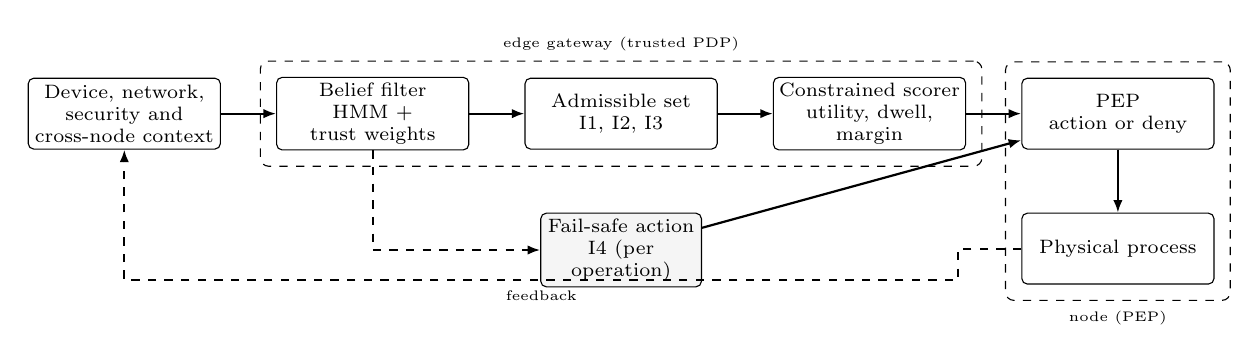
\begin{tikzpicture}[
  font=\scriptsize,
  node distance=5mm and 7mm,
  box/.style={draw, rounded corners=2pt, align=center, minimum height=9mm,
              text width=23mm, inner sep=2pt},
  smallbox/.style={draw, rounded corners=2pt, align=center, minimum height=7mm,
                   text width=19mm, inner sep=2pt, fill=black!4},
  arr/.style={-{Latex[length=1.6mm]}, thick},
  darrow/.style={-{Latex[length=1.6mm]}, thick, dashed},
]
\node[box] (ctx) {Device, network, security and cross-node context};
\node[box, right=of ctx] (belief) {Belief filter\\HMM $+$ trust weights};
\node[box, right=of belief] (safe) {Admissible set\\I1, I2, I3};
\node[box, right=of safe] (score) {Constrained scorer\\utility, dwell, margin};
\node[box, right=of score] (pep) {PEP\\action or deny};
\node[box, below=8mm of pep] (proc) {Physical process};
\node[smallbox, below=8mm of safe] (fail) {Fail-safe action\\I4 (per operation)};

\draw[arr] (ctx) -- (belief);
\draw[arr] (belief) -- (safe);
\draw[arr] (safe) -- (score);
\draw[arr] (score) -- (pep);
\draw[arr] (pep) -- (proc);
\draw[darrow] (proc.west) -| ++(-8mm,-4mm) -| (ctx.south)
  node[pos=0.25, below, font=\tiny] {feedback};
\draw[arr] (fail) -- (pep);
\draw[darrow] (belief.south) |- (fail.west);
\node[draw, dashed, rounded corners=3pt, fit=(belief)(safe)(score), inner sep=2mm,
      label={[font=\tiny]above:edge gateway (trusted PDP)}] {};
\node[draw, dashed, rounded corners=3pt, fit=(pep)(proc), inner sep=2mm,
      label={[font=\tiny]below:node (PEP)}] {};
\end{tikzpicture}}
\caption{Control loop. The belief filter and scorer run on the gateway; the PEP
runs on the node. I1/I2 are enforced in the admissible-set constructor and do
not depend on the belief. The fail-safe path is precomputed per operation class.}
\label{fig:architecture}
\end{figure}

\subsection{Belief over latent threat states}
\label{sec:belief}

Let $\Theta=\{\text{benign},\text{recon},\text{DoS},\text{Byzantine},\text{compromised}\}$
and let $b_t(\btheta)=\Prob(\theta_t=\btheta\mid\bx_{1:t})$ be the defender's
belief. The latent state evolves as a stationary Markov chain with transition
matrix $T$, where $\operatorname{diag}(T)=0.82$ and the remaining mass is spread
uniformly over the other four states. The persistence is deliberate: threat
states are episodes, not independent draws, and a filter that ignores persistence
over-reacts to single observations.

For each modality $m$ with coordinate set $I_m$, the emission model is a product
of univariate Gaussians,
\begin{equation}
  L_m(\bx_t\mid\btheta)
  =\prod_{j\in I_m}\frac{1}{\sigma_{\btheta,j}}
    \exp\!\left[-\frac{(x_{t,j}-\mu_{\btheta,j})^2}{2\sigma_{\btheta,j}^2}\right],
  \label{eq:emission}
\end{equation}
with state- and feature-specific means and standard deviations. In this
simulator the likelihood is evaluated at the same parameters that generate the
observations, so the defender is correctly specified by construction and the
calibration and detection results are an oracle-model upper bound, not an
estimate for a misspecified defender. The classes still overlap by design: a DoS episode and a heavily loaded benign node can produce
similar device telemetry, and a Byzantine node can look almost benign except for
cross-node dispersion. The model is intentionally not tuned so that a single
feature separates the classes.

\paragraph{Trust weights.} For each modality we form a \emph{modality posterior}
$q_m(\btheta)\propto \pi_0(\btheta)L_m(\bx_t\mid\btheta)$ using a fixed reference
prior $\pi_0$, and compare it with the device posterior $q_{\mathrm{dev}}$ by
total variation:
\begin{equation}
  \tau_m = \tfrac12\lVert q_m-q_{\mathrm{dev}}\rVert_1 .
  \label{eq:tv}
\end{equation}
The weight is a logistic gate
\begin{equation}
  \tilde w_m = \frac{1}{1+\exp[(\tau_m-\tau_{\mathrm{TV}})/s_{\mathrm{TV}}]},
  \qquad \tilde w_{\mathrm{dev}}=\tilde w_{\mathrm{cross}}=1 ,
  \label{eq:weight}
\end{equation}
so a modality whose posterior has drifted far from the attestation anchor is
discarded, while the device anchor and the dispersion signal are always kept.
The weight is updated asymmetrically,
\begin{equation}
  w_{m,t}=
  \begin{cases}
    0.2\,w_{m,t-1}+0.8\,\tilde w_m, & \tilde w_m<w_{m,t-1},\\
    0.9\,w_{m,t-1}+0.1\,\tilde w_m, & \text{otherwise},
  \end{cases}
  \label{eq:asym}
\end{equation}
which distrusts quickly (80\,\% of the new evidence) and restores slowly
(10\,\%). Slow restoration prevents a brief clean observation from undoing a
sustained inconsistency.

\paragraph{Fusion.} The fused belief is a forward HMM update with weighted
modality likelihoods:
\begin{equation}
  b_t(\btheta)=\frac{1}{Z_t}
  \Big[\sum_{\btheta'}T_{\btheta'\btheta}\,b_{t-1}(\btheta')\Big]
  \prod_{m\in\mathcal{M}}L_m(\bx_t\mid\btheta)^{w_{m,t}},
  \label{eq:fusion}
\end{equation}
where $Z_t$ normalises the distribution. A separate \emph{uniform-fusion} belief
uses $w_{m,t}=1$ for all modalities; it is the ablation that isolates the value
of trust weighting. The attack probability is
$\attack_t=b_t(\text{DoS})+b_t(\text{Byzantine})+b_t(\text{compromised})$;
reconnaissance is tracked but excluded from the serious-attack mass because it
does not by itself justify a hard restriction.

\paragraph{Consistency score.} For monitoring and for I3 we also need a
belief-free signal. Let $d_t$ be the cross-node dispersion and let
\begin{equation}
  s_t=\max\Big\{\max_{m}\tau_m,\;
  \operatorname{clip}\!\left(\frac{d_t-d_0}{d_1},0,1\right)\Big\},
  \label{eq:consistency}
\end{equation}
with $d_0,d_1$ calibrated from benign traffic. The first term catches a modality
that disagrees with the device anchor; the second catches a colluding minority
that shifts the cross-node spread even when every individual modality looks
plausible. This score is used for detection metrics and as a diagnostic; it is
not the safety mechanism.

\subsection{Action lattice, detection and utility}
\label{sec:utility}

An action $a=(a_{\mathrm{auth}},a_{\mathrm{cry}},a_{\mathrm{ids}},a_{\mathrm{rate}},a_{\mathrm{ttl}})$
is a point in the 243-element lattice. For a malicious request, the probability
that the action detects it is the complement of the probability that every layer
misses:
\begin{equation}
  p_{\mathrm{det}}(\btheta,a)=1-\prod_{\ell}\big(1-p_{\ell}(\btheta,a_\ell)\big),
  \label{eq:detect}
\end{equation}
with base validation, authentication, inspection and rate-limit terms. The
state-dependent multipliers make inspection less effective against a Byzantine
or compromised node (the adversary knows the signatures), and the authentication
term rewards attestation over bearer tokens. For a legitimate request, the
false-positive probability $p_{\mathrm{fp}}(a)$ is the union of the same layers'
false-alarm probabilities.

Let $V_{\op}$ be the value of a granted legitimate request, $D_{\op}$ the damage
of a granted malicious one, and $C_{\op}$ the cost of denying a legitimate
request. With $p_{\mathrm{mal}}(\btheta)=\Prob(\text{request is malicious}\mid\btheta)$,
the expected utility of action $a$ for operation $\op$ in state $\btheta$ is
\begin{equation}
\begin{aligned}
  U_{\op}(\btheta,a)={}&
  p_{\mathrm{mal}}(\btheta)\big[-(1-p_{\mathrm{det}}(\btheta,a))D_{\op}\big]\\
  &+(1-p_{\mathrm{mal}}(\btheta))\big[V_{\op}(1-p_{\mathrm{fp}}(a))-C_{\op}p_{\mathrm{fp}}(a)\big].
\end{aligned}
  \label{eq:utility}
\end{equation}
Safety-critical operations are never malicious in the model, so
$p_{\mathrm{mal}}=0$ for them; the design question there is availability, not
malice. The action score adds the systems cost:
\begin{equation}
  S_{\op}(a;b_t)=b_t^{\top}U_{\op}(\cdot,a)
  -\lambda_L\ell(a)-\lambda_E e(a),
  \label{eq:score}
\end{equation}
where $\ell(a)$ and $e(a)$ are latency and energy, and $\lambda_L,\lambda_E$
convert them to utility units. The realised utility used for reporting adds one
further term, $\rho\,\ind{a\not\models\mathrm{I1}\land a\neq\textsc{Deny}}$
with $\rho=6.0$, which prices a granted action that falls below the floor. This
term is not part of the controller's score---the controller cannot select such
an action---and it exists so that the utility metric does not reward a violation
that the invariants forbid. Denying has score
$-(1-p_{\mathrm{mal}}^{\mathrm{req}})C_{\op}$ with
$p_{\mathrm{mal}}^{\mathrm{req}}=(1-b_t(\text{benign}))P_{\mathrm{malicious}}$:
denying is cheap when the request is likely malicious, but not free when
legitimate traffic is still arriving. This request-level term is important; an
epoch-level denial heuristic over-denies mixed traffic.

\subsection{Admissible set and constrained objective}
\label{sec:admissible}

For operation $\op$ and belief $b$, the admissible set is
\begin{equation}
  \Asafe(\op,b)=\{a\in\Aspace:\; a\models \mathrm{I1}(\op)\land \mathrm{I2}(\op)
  \land \mathrm{I3}(\op,b)\},
  \label{eq:admissible}
\end{equation}
where I1/I2 are the unconditional floors and I3 is the belief-conditional
restriction. Deny is a separate action, admissible only when
$\op\neq\text{safety}$. The controller solves, at each request,
\begin{equation}
  a_t^{\star}=\argmax_{a\in\Asafe(\op,\attack_t)\cup\mathcal{D}(\op)}
  \Big[S_{\op}(a;b_t)-\gamma\,\ind{a\neq a_{t-1}}\Big],
  \label{eq:objective}
\end{equation}
where $\mathcal{D}(\op)$ is the deny singleton for non-safety operations and
$\gamma$ is the switching penalty. The objective is myopic by design: the belief
already carries the temporal state, and a receding-horizon planner would add
latency without changing the safety argument.

\begin{proposition}[Invariant dominance and non-emptiness]
\label{prop:dominance}
For every operation $\op$ and every belief $b\in\Delta(\Theta)$, the set
$\Asafe(\op,b)$ is non-empty. It contains the maximal posture
$a_{\max}=(\text{attestation},\text{Ascon},\text{deep},\text{10/s},\text{10\,s})$,
which satisfies I1, I2 and I3. Consequently, any action returned by
\eqref{eq:objective} is in $\Asafe$, and the fail-safe fallback in I4 is always
defined.
\end{proposition}

\begin{proof}
At $a_{\max}$ the authentication level is 3, the AEAD level is 2, the inspection
level is 2, the rate-limit level is 2 and the freshness level is 2. I1 requires
authentication $\ge 2$, AEAD, freshness $\ge 1$ and inspection $\ge 1$; I2
requires authentication $\ge 2$, inspection $\ge 2$ and freshness $\ge 1$; I3
can only add lower bounds at or below these levels. Hence $a_{\max}$ satisfies
all three for every $\op$ and every $b$. Selection is restricted to $\Asafe$ by
\eqref{eq:objective}; if the set is empty or the controller times out, the PEP
executes $a_{\max}$ (or the operation-specific safe action), which is also
admissible.
\end{proof}

\begin{proposition}[Structural safety for any belief]
\label{prop:structural}
For any belief sequence $\{b_t\}$, any request that is granted by the controller
uses an action that satisfies I1, and, if the request is safety-critical, I2.
Equivalently, the invariant-violation rate is zero by construction, not by
estimation accuracy.
\end{proposition}

\begin{proof}
A granted request is either (i) the output of \eqref{eq:objective}, which lies
in the admissible set $\Asafe$ for that operation and belief and therefore
satisfies I1 and, for safety-critical operations, I2, or (ii) the I4 fallback,
which is $a_{\max}$ and satisfies the same floors. A denied request is not
granted and therefore cannot violate the floors. The claim holds for an
adversarially chosen belief because no step uses a correctness assumption about
$b_t$.
\end{proof}

\begin{proposition}[Safety liveness]
\label{prop:liveness}
For $\op=\text{safety}$, deny is not in the admissible action set for any belief,
and $\Asafe(\text{safety},b)$ is non-empty. A safety-critical request is
therefore never denied by policy; it can only be denied by a stochastic
mechanism failure (authentication or inspection false positive).
\end{proposition}

\begin{proof}
I4 excludes deny for safety, and \cref{prop:dominance} gives a non-empty
admissible set for every belief. The controller must therefore select an action
from $\Asafe(\text{safety},b)$, and the PEP grants it subject only to the
mechanism's false-positive probability.
\end{proof}

\subsection{Fail-safe enforcement algorithm}
\label{sec:algorithm}

\Cref{alg:controller} combines the belief update, admissible-set construction,
scoring, hysteresis and fallback. The hysteresis state is per operation class:
the controller remembers the previous security level and refuses to de-escalate
while the risk is inside the band $[\tau_{\mathrm{down}},\tau_{\mathrm{up}})$
and the low-risk streak is shorter than the dwell time. A lateral or
de-escalating move must beat the incumbent by a margin $m$; an escalation is
immediate. This asymmetry is intentional: safety is allowed to react quickly,
availability is not.

\begin{algorithm}[t]
\caption{Fail-safe context-adaptive enforcement (per epoch)}
\label{alg:controller}
\begin{algorithmic}[1]
\Require observation $\bx_t$; requests $\mathcal{R}_t$; previous state
$\{(a_{\op},s_{\op})\}_{\op}$; low-risk streak $\ell$
\Ensure actions for all requests
\State $q_m\propto\pi_0\odot L_m(\bx_t)$ for each modality $m$
\State $\tau_m\gets\tfrac12\lVert q_m-q_{\mathrm{dev}}\rVert_1$;\quad
       $\tilde w_m\gets\sigma((\tau_{\mathrm{TV}}-\tau_m)/s_{\mathrm{TV}})$
\State $w_t\gets\textsc{AsymUpdate}(w_{t-1},\tilde w)$ \Comment{Eq.~\eqref{eq:asym}}
\State $b_t\gets\textsc{Normalise}\big[(T^{\top}b_{t-1})\odot
       \exp(\sum_m w_{m,t}\log L_m)\big]$ \Comment{Eq.~\eqref{eq:fusion}}
\State $\attack_t\gets b_t(\text{DoS})+b_t(\text{Byz})+b_t(\text{comp})$
\State $\ell\gets\ell+1$ if $\attack_t<\tau_{\mathrm{down}}$ else $0$
\ForAll{$(\op,\ldots)\in\mathcal{R}_t$}
  \State $\Asafe\gets\{a:a\models\mathrm{I1}(\op)\land\mathrm{I2}(\op)\land
         \mathrm{I3}(\op,\attack_t)\}$
  \State $\mathcal{C}\gets\Asafe$;\quad
         if $\op\neq\text{safety}$ then $\mathcal{C}\gets\mathcal{C}\cup\{\textsc{Deny}\}$
  \If{$\mathcal{C}=\emptyset$}
     \State $a^{\star}\gets\textsc{SafeFallback}(\op)$ \Comment{I4}
  \Else
     \State $a^{\star}\gets\argmax_{a\in\mathcal{C}}S_{\op}(a;b_t)-\gamma\ind{a\neq a_{\op}}$
     \State apply dwell floor and margin $m$ to $a^{\star}$
  \EndIf
  \State enforce $a^{\star}$ (or deny if $a^{\star}=\textsc{Deny}$)
  \State update $(a_{\op},s_{\op})$
\EndFor
\end{algorithmic}
\end{algorithm}

\paragraph{Complexity.} The belief update is $O(|\Theta|^2+|\mathcal{M}||\Theta|)$
per epoch, the admissible-set construction is $O(|\Aspace|)$, and scoring is
$O(|\Aspace|)$ per request. With $|\Aspace|=243$ and $|\Theta|=5$, the whole
decision is a few thousand floating-point operations; \cref{sec:evaluation}
shows that it is dominated by the cryptographic mechanisms it selects, not by
the controller.

\paragraph{Why these choices.}
The device modality is the anchor because it is the only context source that is
attested by the node itself; an attacker who controls the network can make the
network and security modalities agree with each other, but not with a value
signed by the device. The cross-node dispersion is kept at full weight because a
colluding minority cannot hide the spread it creates without controlling the
majority. This anchor is an explicit trust assumption: the \texttt{tee}
scenario removes it, and the belief is expected to fail there. Asymmetric trust is a deliberate bias: a false distrust costs some
utility, while a false trust can cost a physical action. The utility margin is
the analogue of a Schmitt trigger; it converts small belief fluctuations into
stability without hiding large ones.

\section{Implementation}
\label{sec:implementation}

\subsection{Simulator and reproducibility}
\label{sec:sim-implementation}

The evaluation harness is a discrete-time simulator written in Python\,3.14 with
NumPy\,2.5 and SciPy\,1.18. It generates a 24-node deployment with the tier mix
of \cref{sec:system-model}, a latent threat state, four context modalities and
per-request access decisions. Each run has 2{,}000 epochs; ten seeds are used for
every scenario, and all ten policies are replayed against the byte-identical
observation and request stream generated for that seed and scenario. Comparisons
are therefore paired, and a policy cannot gain by seeing a different sequence of
requests. The full matrix is 800 policy runs (10 seeds $\times$ 8 scenarios
$\times$ 10 policies) and completes in about 50 seconds on eight cores.

The simulator is \emph{parameterised}, not a replay. The observation model, the
transition matrix and the attack processes are explicit; no raw packet capture is
loaded at run time. The public IoT-23 capture is used offline to calibrate one
prior (the benign-to-malicious network-intensity contrast) and is documented in
\cref{sec:trace}. This distinction is deliberate: a simulator that claims to
replay a dataset but generates random numbers is not reproducible, and a
trace-driven evaluation would answer a different question (can the monitor
recognise known attack signatures?) than the one asked here (does the controller
remain safe when the context is adversarially chosen?).

\subsection{Scenarios and policies}
\label{sec:scenarios}

The eight scenarios share the same node topology and request process; they
differ in the latent state process and the poisoning channel.

\begin{description}
  \item[None.] Benign operation with occasional reconnaissance. This is the
  utility reference, not a safety test.
  \item[DoS.] Three non-overlapping attack windows in which the latent state is
  DoS; the network and security modalities show congestion and inspection
  failures. No context spoofing is applied, so the attack is observable.
  \item[Downgrade.] The same windows, but the adversary moves the network and
  security modalities toward the benign distribution while leaving the attested
  device modality and the cross-node dispersion intact. Physical effects remain,
  but the network evidence is consistent with a calm plant. This is the in-model
  poisoning attack: it assumes the anchor is trustworthy.
  \item[TEE.] An explicit out-of-model stress test in which the adversary also
  spoofs the attested device modality, i.e.\ the node's trusted execution
  environment is assumed subverted. It is the only scenario that instantiates
  the fifth latent state (compromised); the other attack scenarios use DoS,
  Byzantine or no serious state. This scenario exists to separate two claims:
  the invariant guarantee, which still holds, from belief quality, which does
  not. It is not used to argue that the architecture detects a TEE compromise.
  \item[Energy.] The adversary inflates the apparent threat: the network and
  security modalities look like an attack while the plant is benign. The goal is
  denial-of-sleep and over-provisioning.
  \item[Byzantine.] Ten of 24 nodes collude and report fabricated benign context.
  The honest majority still determines the median for most features, but the
  cross-node dispersion rises. This tests aggregation robustness, not majority
  capture.
  \item[Resonant.] The adversary alternates downgrade and energy poisoning at a
  period close to the controller's dwell time, attempting to force posture
  thrashing.
  \item[Adaptive.] The adversary starts with partial spoofing, increases the
  spoofed fraction over the first 600 epochs, and then holds the anomaly score
  just below the public point-estimate threshold (0.55). It uses the published
  policy parameters but does not solve the defender's POMDP.
\end{description}

The ten policies are: Static-High (always the strongest posture, with Ascon at
the AEAD level), Static-Med (a uniform middle posture, raised to each
operation's floor), Static-Low (always the weakest), Threshold-CAAC (a
univariate point-estimate anomaly threshold on the same feature the attacker
manipulates, raised to the structural floor; a multivariate or learned detector
is not evaluated, which is a limitation of the baseline set), Risk-Only
(Bayesian belief, no invariants), Invariant-Only
(invariants, no belief; uses the anomaly point estimate), Full$-$Hyst (full
controller without hysteresis or margin), Full$-$Cons (full controller with
uniform modality fusion), Full (the proposed controller) and Oracle (knows the
latent state). Static-High and Static-Med use the same Ascon primitive as the
adaptive policies, so the comparison is not confounded by cipher choice. The
deliberately unconstrained baselines (Static-Low, Risk-Only) do not install the
node-side PEP re-check; every policy that claims the invariant guarantee does.
Making the unconstrained baselines structurally safe would erase the
counterfactual that RQ1 measures.

\subsection{Analytical cost model}
\label{sec:cost-model}

Latency and energy are estimated from per-layer operation costs rather than
measured on silicon. For action
$a=(a_{\mathrm{auth}},a_{\mathrm{cry}},a_{\mathrm{ids}},a_{\mathrm{rate}},a_{\mathrm{ttl}})$,
\begin{equation}
  \ell(a)=\ell_0+\sum_{\ell}\ell_{\ell}(a_\ell),\qquad
  e(a)=e_0+\sum_{\ell}e_{\ell}(a_\ell),
  \label{eq:cost}
\end{equation}
where the per-layer constants are derived from datasheet-level operation counts
for the three tiers and $\ell_0,e_0$ cover request validation. The tier
multipliers are $1.00$, $0.60$ and $0.35$ for Class-1, Class-2 and gateway
respectively, and the reported latency uses the tier distribution of the
deployment. The resulting numbers are \emph{analytical estimates}; they are
useful for comparing postures and for checking that the controller fits an MCU
budget, but they are not a substitute for a hardware measurement. SRAM and flash
footprints are likewise model estimates: 9--14\,KB SRAM and 58--86\,KB flash
depending on whether the policy needs the belief filter.

The cost model is intentionally coarse. Its role is to make the utility
trade-off non-trivial (stronger actions must buy enough detection to justify
their latency and energy), not to predict a specific board's power draw. A
deployment would replace \eqref{eq:cost} with a measured profile; the controller
only consumes the resulting scalar costs.

\subsection{Verification}
\label{sec:verification}

The invariant layer is verified exhaustively rather than sampled. A unit test
enumerates all 243 actions for each of the four operation classes and checks
that the structural mask matches the independent restatement of I1/I2, that the
conditional mask is a subset of the structural mask for a 41-point grid of
$\attack\in[0,1]$, and that the admissible set is never empty. A second test
runs all adaptive policies on a real stream and asserts that no emitted action
violates I1/I2. Belief normalisation, trust bounds, AUC/TPR helpers, paired
determinism and the trace-calibration consistency are covered by 23 tests, all
passing. These tests do not prove the cryptographic mechanisms; they prove that
the decision layer never selects an action outside the declared envelope.

\section{Evaluation}
\label{sec:evaluation}

\subsection{Protocol}
\label{sec:eval-protocol}

Every number in this section is produced by \texttt{make\_paper\_assets.py} from
\texttt{results/main.csv}; the manuscript does not contain a typed experimental
value. The matrix is $10$ seeds $\times$ $8$ scenarios $\times$ $10$ policies
$=800$ runs of $2{,}000$ epochs each, and all policies replay the same
observation and request stream for a given seed and scenario, so every
comparison is paired. \Cref{tab:params} lists the implementation parameters and
their values as read from the simulator.

For each policy we report six quantities. \emph{Invariant violations per
1{,}000 decisions} (IVR) counts granted requests whose action falls below the
I1/I2 floor; because I1 is an actuation envelope and I2 a safety envelope, this
metric is meaningful only for actuation and safety requests, and we report the
per-operation breakdown in \cref{tab:ivr-byop}. \emph{Malicious-grant rate}
counts malicious requests that were granted, whether or not the action satisfied
I1/I2; it is the residual exposure that survives the invariant layer.
\emph{False-denial rate} is the fraction of legitimate non-safety requests
denied. \emph{Safety-denial rate} is the fraction of safety-critical requests
denied. \emph{Mission utility} is the normalised net value from
\eqref{eq:utility} and \eqref{eq:score}, including energy and latency costs and,
for any granted action below the floor, the violation penalty $\rho=6.0$.
\emph{Calibration} is the Brier score and expected calibration error of the
belief each policy acts on. Unless stated otherwise, an ``attack mean'' is the
unweighted mean over the seven attack scenarios (DoS, downgrade, TEE, energy,
Byzantine, resonant, adaptive); the benign scenario is excluded from attack
aggregates because it contains no serious attack state.

Statistical comparisons aggregate each seed over the seven attack scenarios and
apply a two-sided Wilcoxon signed-rank test ($n=10$) against Full, with Holm
correction within each metric across the four baselines
(\cref{tab:stats}). With ten pairs the test is deliberately conservative; the smallest attainable
two-sided $p$-value is $0.00195$, so every $p_{\text{Holm}}=0.008$ in
\cref{tab:stats} is at the resolution floor and should be read as sign
consistency across seeds rather than as a precise significance level. We report
effect sizes next to $p$-values and do not treat a difference that fails to reach
the $0.05$ level as evidence of equivalence.

% Generated by make_paper_assets.py from simulator.py constants.
\begin{table}[t]
\centering
\small
\caption{Simulation and controller parameters. Values are read from the
implementation, not typed into the manuscript.}
\label{tab:params}
\resizebox{\textwidth}{!}{%
\begin{tabular}{lll}
\toprule
Group & Parameter & Value \\
\midrule
Deployment & nodes / seeds / epochs / policy runs & 24, 10, 2{,}000, 800 \\
Byzantine fraction & colluding nodes $f$ & 10/24 = 0.42 \\
Latent states & benign, recon, DoS, Byzantine, compromised & 5 \\
HMM persistence & $\operatorname{diag}(T)$ & 0.82 \\
Action lattice & $|\mathcal{A}|$ & 243 \\
Prior malice & $P_{\mathrm{malicious}}$ & 0.35 \\
Base detection & $p_{\mathrm{base}}$ & 0.05 \\
Auth detection & token / mutual / attest & 0.02, 0.18, 0.45 \\
IDS detection & off / header / deep & 0.00, 0.45, 0.70 \\
Rate-limit detection & off / 50 / 10 per s & 0.00, 0.15, 0.40 \\
Escalation & $\tau_{\mathrm{up}}$ & 0.60 \\
De-escalation & $\tau_{\mathrm{down}}$ & 0.30 \\
Conditional floor & $\tau_{\mathrm{risk}}$ & 0.55 \\
Strong floor & $\tau_{\mathrm{high}}$ & 0.90 \\
Dwell & epochs & 25 \\
Switch margin & $m$ & 0.06 \\
Trust midpoint / slope & $\tau_{\mathrm{TV}}$ / $s_{\mathrm{TV}}$ & 0.25 / 0.06 \\
Dispersion floor / span & $d_0$ / $d_1$ & 0.09 / 0.16 \\
Cost weights & $\lambda_E$ / $\lambda_L$ / $\gamma$ & 0.15 / 0.02 / 0.05 \\
Safety penalty & $\rho$ & 6.0 \\
\bottomrule
\end{tabular}}
\end{table}


\subsection{RQ1: Do hard invariants eliminate unsafe downgrades?}
\label{sec:rq1}

\Cref{tab:ivr} answers RQ1 directly. Every policy that enforces I1/I2 records
exactly $0.00$ invariant violations per $1{,}000$ decisions in all eight
scenarios. Static-High is zero because it always selects the strongest posture;
Static-Med is zero because it is a fixed mid-point that is raised to each
operation's structural floor; Threshold, Invariant-Only, Full$-$Hyst, Full$-$Cons,
Full and Oracle are zero because they install the node-side PEP re-check. The two policies that do not install
it violate the floor heavily: Static-Low at $393.31$ per $1{,}000$ and Risk-Only
at $327.41$, with attack-scenario values between $303.4$ and $403.9$. Risk-Only is
the informative case: it is a full Bayesian belief controller with the same
trust-weighted estimator as Full, it is granted the same belief stream, and it
still violates the floor at roughly the same rate as a policy that ignores risk
altogether, because nothing in its objective is non-negotiable. Adding the
invariant layer and the PEP re-check to that same estimator removes the
violations entirely.

The zero is structural, not statistical. \Cref{prop:structural} shows that a
granted actuation or safety request is either the constrained argmax, which lies
in $\Asafe$, or the I4 fallback $a_{\max}$, which also lies in $\Asafe$; the proof
makes no assumption about $b_t$. The experiment is a check on the implementation
of that argument, not a measurement of how often the estimator happens to be
right. The strongest empirical support is the \texttt{tee} scenario: Full's
belief is badly wrong there (Brier $0.437$), its utility drops to $0.058$---the
lowest of any attack scenario---and its malicious-grant rate rises to $0.473$---yet
its IVR stays at zero, because the belief can only remove actions from the
admissible set, not add them.

Two baselines also achieve zero IVR, and it is worth being explicit about why
this does not make the invariant layer redundant. Static-High never leaves the
strongest posture, and Static-Med is raised to the floor for each operation;
neither adapts. Threshold is zero only
because we implemented it with the same structural floor
(\texttt{STRUCT\_FLOOR}) rather than as a naive point-estimate threshold; without
that floor it would inherit the violation behaviour of Risk-Only, since it selects
actions from the unconstrained lattice when the score is below threshold. The
contribution of RQ1 is therefore not ``zero IVR'' in isolation but zero IVR
\emph{while adapting}, with the belief free to be wrong.

\Cref{tab:ivr-byop} makes the scope of the claim explicit. Read and write have no
structural floor by design, so their IVR is zero for every policy and says
nothing about posture strength; the guarantee constrains actuation and safety
traffic. On those classes the unconstrained baselines violate almost every
decision in an attack window ($979.81$ actuation and $996.76$ safety per
$1{,}000$ for Static-Low; $778.00$ and $996.76$ for Risk-Only), while every
PEP-enforcing policy records zero.

\begin{figure}[t]
\centering
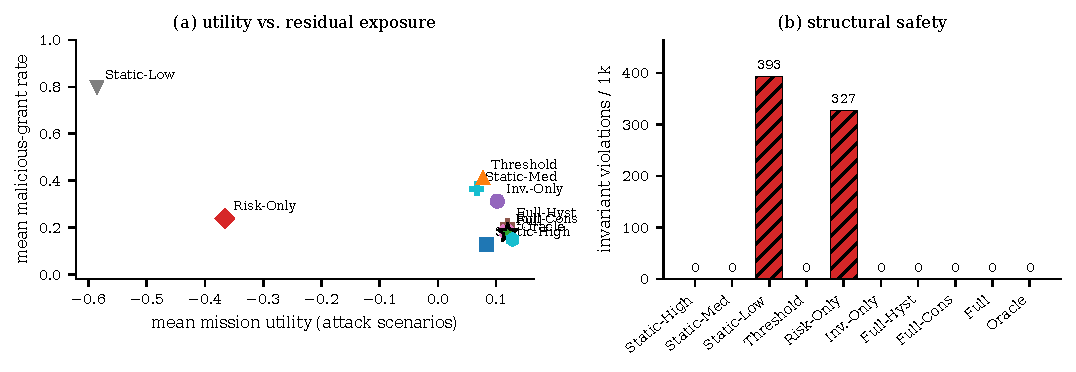
\includegraphics[width=\linewidth]{figures/fig_tradeoff.pdf}
\caption{(a) Mean attack-scenario utility against mean malicious-grant rate;
right and down is better. (b) Invariant violations per $1{,}000$ decisions.
Bars at zero are policies that install the PEP re-check; the two nonzero,
hatched bars are the unconstrained baselines. Static-High is safe and cheap in exposure
but sits at low utility and high false denial; Full keeps zero violations at
higher utility, at the cost of residual exposure concentrated in the
out-of-model TEE scenario.}
\label{fig:tradeoff}
\end{figure}

% Generated by make_paper_assets.py — do not edit by hand; regenerate.
\begin{table*}[t]
\centering
\scriptsize
\setlength{\tabcolsep}{3.0pt}
\caption{Invariant violations per 1,000 decisions (mean $\pm$ std over 10 seeds). A violation is a granted request whose action falls below the I1/I2 floor; zero is the design target and is achieved by every policy that enforces the unconditional invariants.}
\label{tab:ivr}
\resizebox{\textwidth}{!}{%
\begin{tabular}{lccccccccc}
\toprule
Policy & None & DoS & Down. & TEE & Energy & Byz. & Reson. & Adapt. & Attack mean \\
\midrule
Static-High & 0.00\,$\pm$\,0.00 & 0.00\,$\pm$\,0.00 & 0.00\,$\pm$\,0.00 & 0.00\,$\pm$\,0.00 & 0.00\,$\pm$\,0.00 & 0.00\,$\pm$\,0.00 & 0.00\,$\pm$\,0.00 & 0.00\,$\pm$\,0.00 & 0.00 \\
Static-Med & 0.00\,$\pm$\,0.00 & 0.00\,$\pm$\,0.00 & 0.00\,$\pm$\,0.00 & 0.00\,$\pm$\,0.00 & 0.00\,$\pm$\,0.00 & 0.00\,$\pm$\,0.00 & 0.00\,$\pm$\,0.00 & 0.00\,$\pm$\,0.00 & 0.00 \\
Static-Low & 352.74\,$\pm$\,7.01 & 402.54\,$\pm$\,12.16 & 402.85\,$\pm$\,9.76 & 398.36\,$\pm$\,8.86 & 347.03\,$\pm$\,6.62 & 396.10\,$\pm$\,6.47 & 402.40\,$\pm$\,12.26 & 403.87\,$\pm$\,9.81 & 393.31 \\
Threshold & 0.00\,$\pm$\,0.00 & 0.00\,$\pm$\,0.00 & 0.00\,$\pm$\,0.00 & 0.00\,$\pm$\,0.00 & 0.00\,$\pm$\,0.00 & 0.00\,$\pm$\,0.00 & 0.00\,$\pm$\,0.00 & 0.00\,$\pm$\,0.00 & 0.00 \\
Risk-Only & 352.05\,$\pm$\,7.04 & 309.44\,$\pm$\,8.71 & 309.41\,$\pm$\,9.88 & 391.52\,$\pm$\,8.33 & 342.75\,$\pm$\,6.71 & 326.41\,$\pm$\,6.38 & 303.36\,$\pm$\,5.21 & 308.98\,$\pm$\,5.76 & 327.41 \\
Inv.-Only & 0.00\,$\pm$\,0.00 & 0.00\,$\pm$\,0.00 & 0.00\,$\pm$\,0.00 & 0.00\,$\pm$\,0.00 & 0.00\,$\pm$\,0.00 & 0.00\,$\pm$\,0.00 & 0.00\,$\pm$\,0.00 & 0.00\,$\pm$\,0.00 & 0.00 \\
Full$-$Hyst & 0.00\,$\pm$\,0.00 & 0.00\,$\pm$\,0.00 & 0.00\,$\pm$\,0.00 & 0.00\,$\pm$\,0.00 & 0.00\,$\pm$\,0.00 & 0.00\,$\pm$\,0.00 & 0.00\,$\pm$\,0.00 & 0.00\,$\pm$\,0.00 & 0.00 \\
Full$-$Cons & 0.00\,$\pm$\,0.00 & 0.00\,$\pm$\,0.00 & 0.00\,$\pm$\,0.00 & 0.00\,$\pm$\,0.00 & 0.00\,$\pm$\,0.00 & 0.00\,$\pm$\,0.00 & 0.00\,$\pm$\,0.00 & 0.00\,$\pm$\,0.00 & 0.00 \\
\textbf{Full} & 0.00\,$\pm$\,0.00 & 0.00\,$\pm$\,0.00 & 0.00\,$\pm$\,0.00 & 0.00\,$\pm$\,0.00 & 0.00\,$\pm$\,0.00 & 0.00\,$\pm$\,0.00 & 0.00\,$\pm$\,0.00 & 0.00\,$\pm$\,0.00 & 0.00 \\
\emph{Oracle} & 0.00\,$\pm$\,0.00 & 0.00\,$\pm$\,0.00 & 0.00\,$\pm$\,0.00 & 0.00\,$\pm$\,0.00 & 0.00\,$\pm$\,0.00 & 0.00\,$\pm$\,0.00 & 0.00\,$\pm$\,0.00 & 0.00\,$\pm$\,0.00 & 0.00 \\
\bottomrule
\end{tabular}}
\end{table*}

% Generated by make_paper_assets.py — do not edit by hand; regenerate.
\begin{table}[t]
\centering
\scriptsize
\setlength{\tabcolsep}{3.5pt}
\caption{Invariant violations per 1{,}000 decisions by operation class
(attack-scenario mean over 10 seeds). I1 is an actuation envelope and I2 a
safety envelope, so read and write have no structural floor: a zero there
means the invariant does not constrain that class, not that the action was
strong. The unconstrained baselines violate the actuation and safety floors;
every policy that installs the PEP records zero.}
\label{tab:ivr-byop}
\resizebox{\textwidth}{!}{%
\begin{tabular}{lccc}
\toprule
Policy & read + write & actuate & safety \\
\midrule
Static-Low & 0.00 & 979.81 & 996.76 \\
Risk-Only & 0.00 & 778.00 & 996.76 \\
Threshold & 0.00 & 0.00 & 0.00 \\
Inv.-Only & 0.00 & 0.00 & 0.00 \\
\textbf{Full} & 0.00 & 0.00 & 0.00 \\
\bottomrule
\end{tabular}}
\end{table}


\subsection{RQ2: What is the utility cost of the guarantee?}
\label{sec:rq2}

\Cref{tab:utility,tab:falsedeny,tab:exposure} give the three sides of the
trade-off: mission utility, false denial, and residual malicious grants.
\Cref{fig:tradeoff}(a) plots the first against the third.

\paragraph{Utility.} Full attains $0.120$ mean attack-scenario utility, against
$0.084$ for Static-High, $0.077$ for Threshold, $0.102$ for Invariant-Only and
$-0.366$ for Risk-Only. The paired difference against Static-High is $+0.036$
($p_{\text{Holm}}=0.008$) and against Threshold $+0.043$
($p_{\text{Holm}}=0.008$); against Risk-Only and Static-Low the difference is
$+0.486$ and $+0.706$ respectively (\cref{tab:stats}). The absolute gain over
Static-High is modest, which is the honest reading: a safety floor does not
create value, it prevents a particular kind of loss. The larger gains are against
policies that either deny legitimate traffic or fail to detect malicious traffic.

Full is within $0.005$ of the best non-oracle utility in every attack scenario.
The scenario breakdown is more informative than the mean. Full's advantage over
Static-High is largest under energy inflation ($0.174$ versus $0.122$), and it
also gains under the adaptive attacker ($0.127$ versus $0.089$) and the Byzantine
minority ($0.097$ versus $0.057$), where the trust-weighted belief separates
colluding from honest nodes and tracks slow drift. It is close to the oracle under
DoS ($0.131$ versus $0.132$) and energy inflation ($0.174$ versus $0.186$). It
does not lose to Static-High in the \texttt{tee} scenario ($0.058$ versus
$0.053$), but that comparison is misleading: a spoofed anchor makes both postures
select cheap admissible actions, and the cost appears in residual exposure rather
than in utility. The in-model
downgrade no longer produces a utility loss: Full reaches $0.129$ against $0.090$
for Static-High, because the anchor and dispersion keep the belief calibrated.

\paragraph{False denial.} Full denies $0.027$ of legitimate requests over the
attack scenarios, compared with $0.088$ for Static-High, $0.019$ for Threshold,
and $0.003$ for Static-Low. The low Static-Low number is not an achievement: it
grants almost everything, including $0.798$ of malicious requests. Against
Static-High the reduction in false denial is a factor of three, and it is the
main source of Full's utility advantage. Threshold is slightly better than Full on
this metric but pays for it with a $2.3\times$ higher malicious-grant rate
($0.414$).

\paragraph{Residual exposure.} This is where the design is weakest. Full grants
$0.177$ of malicious requests over the attack scenarios, against $0.127$ for
Static-High, $0.148$ for Oracle, $0.312$ for Invariant-Only, $0.414$ for Threshold
and $0.798$ for Static-Low. Static-High is better because it always buys the
deepest inspection and the strongest authentication; Full buys them only when the
belief or I3 says they are needed. The paired difference of $+0.050$ malicious
grants against Static-High is significant ($p_{\text{Holm}}=0.008$) and goes the
wrong way.

The per-scenario decomposition matters for interpreting that gap. Of the $0.050$,
$0.030$ comes from the single out-of-model \texttt{tee} scenario, where Full
grants $0.473$ against Static-High's $0.265$. Excluding \texttt{tee}, Full is
$0.128$ against $0.104$. The remaining in-model gap is small and concentrated
under Byzantine attack ($0.293$ versus $0.253$), where a colluding minority that
keeps every modality plausible is genuinely hard to separate from honest
neighbours. Under DoS, downgrade, resonant and adaptive attack Full is within
$0.03$ of Static-High. The invariant layer bounds the \emph{worst action} but not
the \emph{detection probability} of that action: an attacker who holds a valid
credential and spoofs a benign context can be granted a request that satisfies I1
and still be malicious. This is a real limitation of a decision-layer
contribution, and we state it as such rather than presenting utility alone.

\begin{figure}[t]
\centering
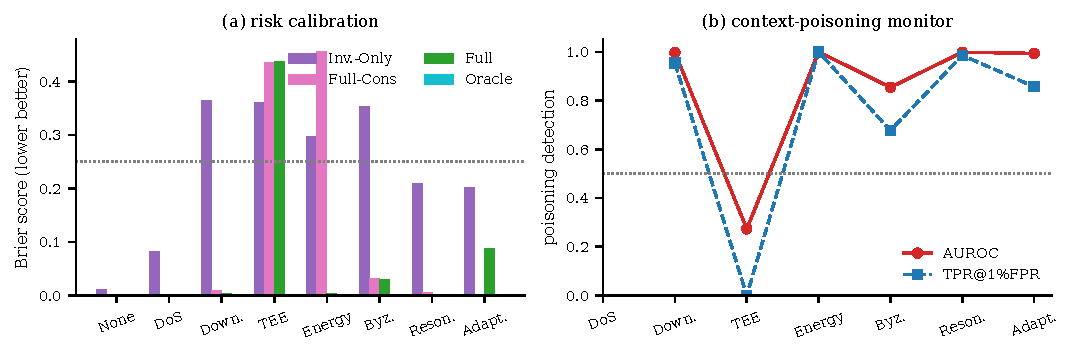
\includegraphics[width=\linewidth]{figures/fig_calibration.pdf}
\caption{(a) Brier score of the risk estimate by scenario for four policies.
(b) Poisoning detection: AUROC and TPR at $1\,\%$ FPR for the consistency
monitor. The \texttt{tee} scenario is the honest negative result: a spoofed
attestation anchor drives both the belief and the monitor below chance. The
in-model downgrade, by contrast, is detected.}
\label{fig:calibration}
\end{figure}

% Generated by make_paper_assets.py — do not edit by hand; regenerate.
\begin{table*}[t]
\centering
\scriptsize
\setlength{\tabcolsep}{3.0pt}
\caption{Mission utility (mean $\pm$ std over 10 seeds; higher is better). Utility normalises value, damage, denial cost, energy and latency by $V_{\max}$; it is negative when denials and damage dominate. Bold marks the best non-oracle policy per scenario.}
\label{tab:utility}
\resizebox{\textwidth}{!}{%
\begin{tabular}{lccccccccc}
\toprule
Policy & None & DoS & Down. & TEE & Energy & Byz. & Reson. & Adapt. & Attack mean \\
\midrule
Static-High & 0.121\,$\pm$\,0.004 & 0.090\,$\pm$\,0.007 & 0.090\,$\pm$\,0.007 & 0.053\,$\pm$\,0.012 & 0.122\,$\pm$\,0.006 & 0.057\,$\pm$\,0.008 & 0.087\,$\pm$\,0.004 & 0.089\,$\pm$\,0.004 & 0.084 \\
Static-Med & 0.162\,$\pm$\,0.003 & 0.064\,$\pm$\,0.015 & 0.065\,$\pm$\,0.013 & 0.025\,$\pm$\,0.017 & 0.162\,$\pm$\,0.004 & 0.033\,$\pm$\,0.016 & 0.057\,$\pm$\,0.009 & 0.062\,$\pm$\,0.011 & 0.067 \\
Static-Low & -0.330\,$\pm$\,0.009 & -0.629\,$\pm$\,0.035 & -0.632\,$\pm$\,0.024 & -0.620\,$\pm$\,0.034 & -0.322\,$\pm$\,0.007 & -0.608\,$\pm$\,0.031 & -0.648\,$\pm$\,0.038 & -0.640\,$\pm$\,0.033 & -0.586 \\
Threshold & 0.183\,$\pm$\,0.003 & 0.108\,$\pm$\,0.010 & 0.060\,$\pm$\,0.016 & 0.028\,$\pm$\,0.018 & 0.155\,$\pm$\,0.006 & 0.039\,$\pm$\,0.017 & 0.084\,$\pm$\,0.009 & 0.068\,$\pm$\,0.012 & 0.077 \\
Risk-Only & -0.331\,$\pm$\,0.009 & -0.316\,$\pm$\,0.012 & -0.318\,$\pm$\,0.010 & -0.599\,$\pm$\,0.036 & -0.323\,$\pm$\,0.007 & -0.376\,$\pm$\,0.012 & -0.313\,$\pm$\,0.009 & -0.319\,$\pm$\,0.008 & -0.366 \\
Inv.-Only & 0.179\,$\pm$\,0.003 & 0.121\,$\pm$\,0.009 & 0.090\,$\pm$\,0.014 & \textbf{0.059\,$\pm$\,0.023} & 0.167\,$\pm$\,0.005 & 0.048\,$\pm$\,0.017 & 0.115\,$\pm$\,0.006 & 0.115\,$\pm$\,0.008 & 0.102 \\
Full$-$Hyst & \textbf{0.184\,$\pm$\,0.003} & \textbf{0.135\,$\pm$\,0.006} & \textbf{0.133\,$\pm$\,0.008} & 0.030\,$\pm$\,0.018 & \textbf{0.179\,$\pm$\,0.004} & \textbf{0.100\,$\pm$\,0.011} & \textbf{0.128\,$\pm$\,0.005} & \textbf{0.132\,$\pm$\,0.005} & 0.119 \\
Full$-$Cons & 0.179\,$\pm$\,0.003 & 0.131\,$\pm$\,0.006 & 0.127\,$\pm$\,0.008 & 0.053\,$\pm$\,0.021 & 0.166\,$\pm$\,0.005 & 0.097\,$\pm$\,0.010 & 0.124\,$\pm$\,0.004 & 0.128\,$\pm$\,0.005 & 0.118 \\
\textbf{Full} & 0.177\,$\pm$\,0.003 & 0.131\,$\pm$\,0.006 & 0.129\,$\pm$\,0.008 & 0.058\,$\pm$\,0.014 & 0.174\,$\pm$\,0.004 & 0.097\,$\pm$\,0.010 & 0.124\,$\pm$\,0.004 & 0.127\,$\pm$\,0.005 & 0.120 \\
\emph{Oracle} & 0.182\,$\pm$\,0.003 & 0.132\,$\pm$\,0.007 & 0.130\,$\pm$\,0.008 & 0.093\,$\pm$\,0.011 & 0.186\,$\pm$\,0.004 & 0.100\,$\pm$\,0.010 & 0.126\,$\pm$\,0.004 & 0.130\,$\pm$\,0.005 & 0.128 \\
\bottomrule
\end{tabular}}
\end{table*}

% Generated by make_paper_assets.py — do not edit by hand; regenerate.
\begin{table*}[t]
\centering
\scriptsize
\setlength{\tabcolsep}{3.0pt}
\caption{False-denial rate on legitimate requests (mean $\pm$ std over 10 seeds; lower is better). Bold marks the best non-oracle policy per scenario.}
\label{tab:falsedeny}
\resizebox{\textwidth}{!}{%
\begin{tabular}{lccccccccc}
\toprule
Policy & None & DoS & Down. & TEE & Energy & Byz. & Reson. & Adapt. & Attack mean \\
\midrule
Static-High & 0.087\,$\pm$\,0.004 & 0.090\,$\pm$\,0.004 & 0.089\,$\pm$\,0.004 & 0.087\,$\pm$\,0.009 & 0.089\,$\pm$\,0.003 & 0.089\,$\pm$\,0.005 & 0.086\,$\pm$\,0.004 & 0.085\,$\pm$\,0.005 & 0.088 \\
Static-Med & 0.024\,$\pm$\,0.002 & 0.026\,$\pm$\,0.002 & 0.024\,$\pm$\,0.003 & 0.024\,$\pm$\,0.004 & 0.025\,$\pm$\,0.002 & 0.025\,$\pm$\,0.002 & 0.024\,$\pm$\,0.003 & 0.024\,$\pm$\,0.003 & 0.024 \\
Static-Low & \textbf{0.003\,$\pm$\,0.000} & \textbf{0.003\,$\pm$\,0.001} & \textbf{0.003\,$\pm$\,0.001} & \textbf{0.003\,$\pm$\,0.001} & \textbf{0.003\,$\pm$\,0.001} & \textbf{0.003\,$\pm$\,0.001} & \textbf{0.003\,$\pm$\,0.001} & \textbf{0.003\,$\pm$\,0.001} & 0.003 \\
Threshold & 0.007\,$\pm$\,0.001 & 0.030\,$\pm$\,0.002 & 0.008\,$\pm$\,0.002 & 0.008\,$\pm$\,0.002 & 0.044\,$\pm$\,0.004 & 0.008\,$\pm$\,0.002 & 0.024\,$\pm$\,0.003 & 0.012\,$\pm$\,0.002 & 0.019 \\
Risk-Only & 0.003\,$\pm$\,0.001 & 0.017\,$\pm$\,0.002 & 0.016\,$\pm$\,0.003 & 0.004\,$\pm$\,0.001 & 0.010\,$\pm$\,0.002 & 0.013\,$\pm$\,0.001 & 0.017\,$\pm$\,0.003 & 0.015\,$\pm$\,0.003 & 0.013 \\
Inv.-Only & 0.015\,$\pm$\,0.003 & 0.030\,$\pm$\,0.003 & 0.013\,$\pm$\,0.004 & 0.014\,$\pm$\,0.002 & 0.030\,$\pm$\,0.004 & 0.011\,$\pm$\,0.002 & 0.027\,$\pm$\,0.003 & 0.017\,$\pm$\,0.002 & 0.020 \\
Full$-$Hyst & 0.012\,$\pm$\,0.003 & 0.027\,$\pm$\,0.002 & 0.024\,$\pm$\,0.003 & 0.011\,$\pm$\,0.003 & 0.017\,$\pm$\,0.003 & 0.028\,$\pm$\,0.004 & 0.026\,$\pm$\,0.003 & 0.024\,$\pm$\,0.003 & 0.022 \\
Full$-$Cons & 0.018\,$\pm$\,0.004 & 0.032\,$\pm$\,0.003 & 0.027\,$\pm$\,0.003 & 0.015\,$\pm$\,0.003 & 0.032\,$\pm$\,0.003 & 0.026\,$\pm$\,0.002 & 0.029\,$\pm$\,0.003 & 0.028\,$\pm$\,0.003 & 0.027 \\
\textbf{Full} & 0.020\,$\pm$\,0.004 & 0.032\,$\pm$\,0.003 & 0.029\,$\pm$\,0.003 & 0.018\,$\pm$\,0.004 & 0.023\,$\pm$\,0.003 & 0.026\,$\pm$\,0.002 & 0.031\,$\pm$\,0.003 & 0.029\,$\pm$\,0.004 & 0.027 \\
\emph{Oracle} & 0.013\,$\pm$\,0.002 & 0.031\,$\pm$\,0.004 & 0.029\,$\pm$\,0.003 & 0.026\,$\pm$\,0.004 & 0.008\,$\pm$\,0.001 & 0.025\,$\pm$\,0.003 & 0.029\,$\pm$\,0.002 & 0.026\,$\pm$\,0.003 & 0.025 \\
\bottomrule
\end{tabular}}
\end{table*}

% Generated by make_paper_assets.py — do not edit by hand; regenerate.
\begin{table*}[t]
\centering
\scriptsize
\setlength{\tabcolsep}{3.0pt}
\caption{Residual exposure: fraction of malicious requests granted (mean $\pm$ std over 10 seeds; lower is better). This is not an invariant violation: the action may still satisfy I1/I2, but a credential-holding attacker was not detected. Bold marks the best non-oracle policy per scenario.}
\label{tab:exposure}
\resizebox{\textwidth}{!}{%
\begin{tabular}{lccccccccc}
\toprule
Policy & None & DoS & Down. & TEE & Energy & Byz. & Reson. & Adapt. & Attack mean \\
\midrule
Static-High & \textbf{0.000\,$\pm$\,0.000} & \textbf{0.088\,$\pm$\,0.014} & \textbf{0.091\,$\pm$\,0.011} & \textbf{0.265\,$\pm$\,0.023} & \textbf{0.000\,$\pm$\,0.000} & \textbf{0.253\,$\pm$\,0.021} & \textbf{0.094\,$\pm$\,0.012} & \textbf{0.095\,$\pm$\,0.010} & 0.127 \\
Static-Med & 0.000\,$\pm$\,0.000 & 0.367\,$\pm$\,0.034 & 0.357\,$\pm$\,0.020 & 0.554\,$\pm$\,0.021 & 0.000\,$\pm$\,0.000 & 0.541\,$\pm$\,0.017 & 0.364\,$\pm$\,0.023 & 0.370\,$\pm$\,0.016 & 0.365 \\
Static-Low & 0.000\,$\pm$\,0.000 & 0.931\,$\pm$\,0.011 & 0.931\,$\pm$\,0.007 & 0.928\,$\pm$\,0.012 & 0.000\,$\pm$\,0.000 & 0.938\,$\pm$\,0.010 & 0.926\,$\pm$\,0.012 & 0.932\,$\pm$\,0.014 & 0.798 \\
Threshold & 0.000\,$\pm$\,0.000 & 0.178\,$\pm$\,0.019 & 0.573\,$\pm$\,0.024 & 0.695\,$\pm$\,0.019 & 0.000\,$\pm$\,0.000 & 0.687\,$\pm$\,0.016 & 0.335\,$\pm$\,0.016 & 0.430\,$\pm$\,0.019 & 0.414 \\
Risk-Only & 0.000\,$\pm$\,0.000 & 0.111\,$\pm$\,0.013 & 0.122\,$\pm$\,0.013 & 0.885\,$\pm$\,0.047 & 0.000\,$\pm$\,0.000 & 0.302\,$\pm$\,0.019 & 0.119\,$\pm$\,0.013 & 0.125\,$\pm$\,0.013 & 0.238 \\
Inv.-Only & 0.000\,$\pm$\,0.000 & 0.182\,$\pm$\,0.018 & 0.382\,$\pm$\,0.051 & 0.545\,$\pm$\,0.077 & 0.000\,$\pm$\,0.000 & 0.631\,$\pm$\,0.030 & 0.196\,$\pm$\,0.015 & 0.249\,$\pm$\,0.017 & 0.312 \\
Full$-$Hyst & 0.000\,$\pm$\,0.000 & 0.110\,$\pm$\,0.013 & 0.121\,$\pm$\,0.014 & 0.695\,$\pm$\,0.019 & 0.000\,$\pm$\,0.000 & 0.299\,$\pm$\,0.018 & 0.119\,$\pm$\,0.013 & 0.123\,$\pm$\,0.012 & 0.209 \\
Full$-$Cons & 0.000\,$\pm$\,0.000 & 0.110\,$\pm$\,0.013 & 0.139\,$\pm$\,0.012 & 0.493\,$\pm$\,0.072 & 0.000\,$\pm$\,0.000 & 0.294\,$\pm$\,0.019 & 0.127\,$\pm$\,0.017 & 0.122\,$\pm$\,0.013 & 0.184 \\
\textbf{Full} & 0.000\,$\pm$\,0.000 & 0.111\,$\pm$\,0.013 & 0.120\,$\pm$\,0.015 & 0.473\,$\pm$\,0.063 & 0.000\,$\pm$\,0.000 & 0.293\,$\pm$\,0.019 & 0.119\,$\pm$\,0.013 & 0.123\,$\pm$\,0.012 & 0.177 \\
\emph{Oracle} & 0.000\,$\pm$\,0.000 & 0.110\,$\pm$\,0.013 & 0.113\,$\pm$\,0.012 & 0.296\,$\pm$\,0.022 & 0.000\,$\pm$\,0.000 & 0.285\,$\pm$\,0.020 & 0.116\,$\pm$\,0.015 & 0.118\,$\pm$\,0.010 & 0.148 \\
\bottomrule
\end{tabular}}
\end{table*}

% Generated by make_paper_assets.py. Paired by seed; values are means over the
% seven attack scenarios per seed (n=10). Wilcoxon signed-rank, Holm within metric.
\begin{table}[t]
\centering
\small
\caption{Paired comparison against Full, aggregated over the seven attack scenarios
per seed ($n=10$). $\Delta$ is Full minus baseline; a negative $\Delta$ for
malicious grant and IVR is better. $p_{\text{Holm}}$ is within the metric across
the four baselines. Em dashes mark identical vectors (no test).}
\label{tab:stats}
\begin{tabular}{lcccccc}
\toprule
 & \multicolumn{2}{c}{Utility $\uparrow$} & \multicolumn{2}{c}{Malicious grant $\downarrow$} & \multicolumn{2}{c}{IVR/1k $\downarrow$} \\
\cmidrule(lr){2-3}\cmidrule(lr){4-5}\cmidrule(lr){6-7}
Baseline & $\Delta$ & $p_{\text{Holm}}$ & $\Delta$ & $p_{\text{Holm}}$ & $\Delta$ & $p_{\text{Holm}}$ \\
\midrule
Static-High & +0.036 & 0.008 & +0.050 & 0.008 & 0.000 & -- \\
Threshold & +0.043 & 0.008 & -0.237 & 0.008 & 0.000 & -- \\
Risk-Only & +0.486 & 0.008 & -0.061 & 0.008 & -327.409 & 0.004 \\
Static-Low & +0.706 & 0.008 & -0.621 & 0.008 & -393.308 & 0.004 \\
\bottomrule
\end{tabular}
\end{table}


\subsection{RQ3: Is the belief calibrated under poisoning?}
\label{sec:rq3}

\Cref{tab:calibration,tab:detection} and \cref{fig:calibration} answer RQ3.
The answer is conditional on what the adversary can spoof.

\paragraph{Calibration.} Full's Brier score is $0.002$ under benign operation,
$0.002$ under DoS, $0.003$ under in-model downgrade, $0.003$ under energy
inflation, $0.030$ under Byzantine attack and $0.088$ under the adaptive attacker.
Those are close to the oracle's zero and far below the $0.25$ of an uninformative
forecast. The single failure is the out-of-model \texttt{tee} scenario ($0.437$),
where the anchor itself is moved toward benign and the belief becomes confidently
wrong. The contrast with the earlier intuition is important: a downgrade that
leaves the attested device modality and the cross-node dispersion intact is
\emph{not} a belief failure, because those two signals still carry the attack.

\paragraph{The value of trust weighting.} The ablation isolates the fusion
mechanism. Full$-$Cons uses uniform modality weights and is otherwise identical.
Its Brier score under energy inflation is $0.455$ against $0.003$ for Full, a
factor of about $140$, and $0.436$ under \texttt{tee} against $0.437$---the trust
weighting cannot rescue a scenario in which the adversary moves every modality
coherently, but it almost eliminates the damage when only the network and
security modalities are inflated. Invariant-Only, which replaces the belief with a
point anomaly score, has Brier $0.296$ under energy inflation and $0.354$ under
Byzantine attack; the continuous belief with trust weights is substantially better
in both. The advantage is not uniform: under the adaptive attacker Full$-$Cons is
better calibrated ($0.003$ versus $0.088$), because its conservatism lowers
confidence when the attack is slow. Trust weighting buys robustness to partial
poisoning, not uniformly lower Brier.

\paragraph{Detection.} The consistency monitor detects energy inflation almost
perfectly (AUROC $1.000$, TPR@$1\,\%$FPR $1.000$), resonant pulsing well
($0.999$, $0.986$), the adaptive attacker well ($0.994$, $0.857$), the in-model
downgrade well ($0.997$, $0.954$) and the Byzantine minority moderately
($0.854$, $0.677$). The \texttt{tee} scenario is below chance (AUROC $0.273$,
TPR $0.000$): when the adversary controls every modality including the anchor,
the consistency score is \emph{lower} during the attack than during benign
operation, so a monitor that thresholds disagreement is systematically fooled.
The belief AUROC in that scenario is $0.210$, also below chance.

This result is not a bug to be tuned away; it is the reason the architecture
separates the estimator from the guarantee. If the safety argument depended on
the belief being right, an anchor compromise would be a safety failure. Because I1
and I2 are unconditional, the same scenario produces zero invariant violations and
a bounded (if unsatisfactory) posture. The correct response to
\cref{tab:detection} is to strengthen the unconditional floor, not to add
confidence to a monitor that cannot see the attack; \cref{sec:rq5-floor}
quantifies that trade.

% Generated by make_paper_assets.py — do not edit by hand; regenerate.
\begin{table*}[t]
\centering
\scriptsize
\setlength{\tabcolsep}{3.5pt}
\caption{Calibration of the risk estimate each policy acts on: Brier score and
expected calibration error (mean over 10 seeds; lower is better). Static and
threshold policies have no risk estimate, so they are omitted. Risk-Only and
Full share the same trust-weighted belief, so their calibration rows coincide;
they differ in the admissible set and the PEP re-check.}
\label{tab:calibration}
\resizebox{\textwidth}{!}{%
\begin{tabular}{llcccccccc}
\toprule
Metric & Policy & None & DoS & Down. & TEE & Energy & Byz. & Reson. & Adapt. \\
\midrule
Brier & Risk-Only & 0.002\,$\pm$\,0.001 & 0.002\,$\pm$\,0.000 & 0.003\,$\pm$\,0.001 & 0.437\,$\pm$\,0.041 & 0.003\,$\pm$\,0.001 & 0.030\,$\pm$\,0.006 & 0.002\,$\pm$\,0.001 & 0.088\,$\pm$\,0.024 \\
 & Inv.-Only & 0.010\,$\pm$\,0.000 & 0.082\,$\pm$\,0.006 & 0.364\,$\pm$\,0.021 & 0.360\,$\pm$\,0.033 & 0.296\,$\pm$\,0.029 & 0.354\,$\pm$\,0.036 & 0.209\,$\pm$\,0.014 & 0.202\,$\pm$\,0.020 \\
 & Full$-$Cons & 0.001\,$\pm$\,0.000 & 0.000\,$\pm$\,0.000 & 0.008\,$\pm$\,0.001 & 0.436\,$\pm$\,0.041 & 0.455\,$\pm$\,0.046 & 0.031\,$\pm$\,0.006 & 0.005\,$\pm$\,0.002 & 0.003\,$\pm$\,0.003 \\
 & \textbf{Full} & 0.002\,$\pm$\,0.001 & 0.002\,$\pm$\,0.000 & 0.003\,$\pm$\,0.001 & 0.437\,$\pm$\,0.041 & 0.003\,$\pm$\,0.001 & 0.030\,$\pm$\,0.006 & 0.002\,$\pm$\,0.001 & 0.088\,$\pm$\,0.024 \\
 & \emph{Oracle} & 0.000\,$\pm$\,0.000 & 0.000\,$\pm$\,0.000 & 0.000\,$\pm$\,0.000 & 0.000\,$\pm$\,0.000 & 0.000\,$\pm$\,0.000 & 0.000\,$\pm$\,0.000 & 0.000\,$\pm$\,0.000 & 0.000\,$\pm$\,0.000 \\
\midrule
ECE & Risk-Only & 0.010\,$\pm$\,0.001 & 0.006\,$\pm$\,0.001 & 0.006\,$\pm$\,0.001 & 0.435\,$\pm$\,0.041 & 0.015\,$\pm$\,0.002 & 0.043\,$\pm$\,0.008 & 0.006\,$\pm$\,0.001 & 0.117\,$\pm$\,0.028 \\
 & Inv.-Only & 0.078\,$\pm$\,0.001 & 0.205\,$\pm$\,0.012 & 0.371\,$\pm$\,0.026 & 0.360\,$\pm$\,0.039 & 0.405\,$\pm$\,0.034 & 0.339\,$\pm$\,0.043 & 0.235\,$\pm$\,0.021 & 0.310\,$\pm$\,0.022 \\
 & Full$-$Cons & 0.008\,$\pm$\,0.001 & 0.004\,$\pm$\,0.001 & 0.015\,$\pm$\,0.003 & 0.434\,$\pm$\,0.041 & 0.459\,$\pm$\,0.046 & 0.046\,$\pm$\,0.008 & 0.010\,$\pm$\,0.001 & 0.010\,$\pm$\,0.004 \\
 & \textbf{Full} & 0.010\,$\pm$\,0.001 & 0.006\,$\pm$\,0.001 & 0.006\,$\pm$\,0.001 & 0.435\,$\pm$\,0.041 & 0.015\,$\pm$\,0.002 & 0.043\,$\pm$\,0.008 & 0.006\,$\pm$\,0.001 & 0.117\,$\pm$\,0.028 \\
 & \emph{Oracle} & 0.000\,$\pm$\,0.000 & 0.000\,$\pm$\,0.000 & 0.000\,$\pm$\,0.000 & 0.000\,$\pm$\,0.000 & 0.000\,$\pm$\,0.000 & 0.000\,$\pm$\,0.000 & 0.000\,$\pm$\,0.000 & 0.000\,$\pm$\,0.000 \\
\bottomrule
\end{tabular}}
\end{table*}

% Generated by make_paper_assets.py — do not edit by hand; regenerate.
\begin{table}[t]
\centering
\small
\caption{Context-poisoning detection and belief discrimination by scenario
(mean over 10 seeds). Poison AUROC/TPR use the monitor's consistency score;
belief AUROC uses the Full policy's $P(\text{serious attack})$. Dashes mark
scenarios without poisoned epochs or without a serious-attack state.}
\label{tab:detection}
\begin{tabular}{lcccc}
\toprule
Scenario & Poison AUROC & TPR@1\%FPR & Belief AUROC & Brier (Full) \\
\midrule
None & -- & -- & -- & 0.002 \\
DoS & -- & -- & 1.000 & 0.002 \\
Down. & 0.997 & 0.954 & 1.000 & 0.003 \\
TEE & 0.273 & 0.000 & 0.210 & 0.437 \\
Energy & 1.000 & 1.000 & -- & 0.003 \\
Byz. & 0.854 & 0.677 & 0.997 & 0.030 \\
Reson. & 0.999 & 0.986 & 1.000 & 0.002 \\
Adapt. & 0.994 & 0.857 & 0.995 & 0.088 \\
\bottomrule
\end{tabular}
\end{table}


\subsection{RQ4: Does per-operation fail-safe semantics work?}
\label{sec:rq4}

\Cref{tab:safety} reports denial of safety-critical requests. Full denies
$0.029$ of them over the attack scenarios, against $0.088$ for Static-High and
$0.039$ for Threshold. Static-Low and Risk-Only deny only $0.003$, but they do so
by not enforcing I2: their safety-critical requests are served by weak actions
with low false-positive probability, which is exactly the failure I4 is designed
to prevent. Among policies that enforce I2, Full is tied for the lowest
safety-denial rate because it selects the cheapest action that satisfies the
envelope, rather than the maximal action.

The residual $0.029$ is not a policy denial. Deny is absent from the admissible
set for safety operations by I4, so every one of those denials is a stochastic
authentication or inspection false positive on an otherwise admissible action.
A caveat on scope: safety requests are legitimate in the simulator, so this
measures the mechanism false-positive floor, not an adversary deliberately
trying to suppress a safety action. Goal (ii) of the threat model is therefore
not separately instantiated; doing so would require forged or replayed safety
credentials and is left to future work.
This is the correct failure semantics: the controller does not choose to deny a
safety request, and the invariant layer does not permit it. The absolute level of
$0.029$ is a property of the I2 floor, not of adaptation: any policy that selects
an action at that floor inherits roughly the same mechanism false-positive rate.
What adaptation changes is which admissible action is selected---Full and
Invariant-Only take the cheapest, Threshold a stronger one, and Static-High a
stronger envelope still---so the comparison among floor-enforcing policies is
about the excess strength they buy, not about whether I2 is enforced. The exhaustive
test enumerates all $243$ actions for all four operation classes, checks that the
admissible set is non-empty for a $41$-point grid of $\attack\in[0,1]$, and
asserts that the conditional mask is a subset of the structural mask. A second
test exercises the empty-mask fallback and the PEP re-check, and a third runs
every adaptive policy on a live stream and finds no granted action outside I1/I2.
These tests verify the decision layer, not the cryptographic primitives; the
latter are assumed correct.

The comparison with a global fail-closed policy is implicit in Static-High's
$0.088$: a design that always uses the strongest envelope pays roughly three
times the safety-denial rate of one that selects the cheapest admissible action.
The comparison with a global fail-open policy is Static-Low's $0.003$ at the cost
of $393.31$ invariant violations per $1{,}000$ decisions. Neither global semantics
is acceptable; the per-operation envelope is what allows the controller to be
available for safety traffic without being permissive for actuation.

% Generated by make_paper_assets.py — do not edit by hand; regenerate.
\begin{table*}[t]
\centering
\scriptsize
\setlength{\tabcolsep}{3.5pt}
\caption{Denial rate on safety-critical requests (mean $\pm$ std over 10 seeds;
lower is better). Deny is inadmissible for this operation class (I4), so every
denial is a stochastic authentication/IDS false positive, not a policy choice.
The rate depends on which admissible action is selected inside the I2 floor,
which is why Threshold differs from the policies that select the cheapest one.}
\label{tab:safety}
\resizebox{\textwidth}{!}{%
\begin{tabular}{lccccccccc}
\toprule
Policy & None & DoS & Down. & TEE & Energy & Byz. & Reson. & Adapt. & Attack mean \\
\midrule
Static-High & 0.089\,$\pm$\,0.012 & 0.095\,$\pm$\,0.015 & 0.087\,$\pm$\,0.014 & 0.086\,$\pm$\,0.020 & 0.082\,$\pm$\,0.014 & 0.091\,$\pm$\,0.012 & 0.091\,$\pm$\,0.016 & 0.087\,$\pm$\,0.019 & 0.088 \\
Static-Med & 0.038\,$\pm$\,0.014 & 0.037\,$\pm$\,0.010 & 0.041\,$\pm$\,0.011 & 0.037\,$\pm$\,0.012 & 0.039\,$\pm$\,0.011 & 0.041\,$\pm$\,0.010 & 0.041\,$\pm$\,0.010 & 0.038\,$\pm$\,0.010 & 0.039 \\
Static-Low & 0.002\,$\pm$\,0.003 & 0.003\,$\pm$\,0.003 & 0.002\,$\pm$\,0.002 & 0.004\,$\pm$\,0.003 & 0.004\,$\pm$\,0.005 & 0.003\,$\pm$\,0.003 & 0.004\,$\pm$\,0.004 & 0.003\,$\pm$\,0.002 & 0.003 \\
Threshold & 0.026\,$\pm$\,0.011 & 0.052\,$\pm$\,0.014 & 0.029\,$\pm$\,0.010 & 0.028\,$\pm$\,0.008 & 0.053\,$\pm$\,0.012 & 0.031\,$\pm$\,0.011 & 0.046\,$\pm$\,0.012 & 0.032\,$\pm$\,0.008 & 0.039 \\
Risk-Only & 0.002\,$\pm$\,0.003 & 0.003\,$\pm$\,0.003 & 0.002\,$\pm$\,0.002 & 0.004\,$\pm$\,0.003 & 0.004\,$\pm$\,0.005 & 0.003\,$\pm$\,0.003 & 0.004\,$\pm$\,0.004 & 0.003\,$\pm$\,0.002 & 0.003 \\
Inv.-Only & 0.026\,$\pm$\,0.011 & 0.030\,$\pm$\,0.009 & 0.029\,$\pm$\,0.010 & 0.028\,$\pm$\,0.008 & 0.029\,$\pm$\,0.010 & 0.031\,$\pm$\,0.011 & 0.033\,$\pm$\,0.008 & 0.026\,$\pm$\,0.007 & 0.029 \\
Full$-$Hyst & 0.026\,$\pm$\,0.011 & 0.030\,$\pm$\,0.009 & 0.029\,$\pm$\,0.010 & 0.028\,$\pm$\,0.008 & 0.029\,$\pm$\,0.010 & 0.031\,$\pm$\,0.011 & 0.033\,$\pm$\,0.008 & 0.026\,$\pm$\,0.007 & 0.029 \\
Full$-$Cons & 0.026\,$\pm$\,0.011 & 0.030\,$\pm$\,0.009 & 0.029\,$\pm$\,0.010 & 0.028\,$\pm$\,0.008 & 0.029\,$\pm$\,0.010 & 0.031\,$\pm$\,0.011 & 0.033\,$\pm$\,0.008 & 0.026\,$\pm$\,0.007 & 0.029 \\
\textbf{Full} & 0.026\,$\pm$\,0.011 & 0.030\,$\pm$\,0.009 & 0.029\,$\pm$\,0.010 & 0.028\,$\pm$\,0.008 & 0.029\,$\pm$\,0.010 & 0.031\,$\pm$\,0.011 & 0.033\,$\pm$\,0.008 & 0.026\,$\pm$\,0.007 & 0.029 \\
\emph{Oracle} & 0.026\,$\pm$\,0.011 & 0.030\,$\pm$\,0.009 & 0.029\,$\pm$\,0.010 & 0.028\,$\pm$\,0.008 & 0.029\,$\pm$\,0.010 & 0.031\,$\pm$\,0.011 & 0.033\,$\pm$\,0.008 & 0.026\,$\pm$\,0.007 & 0.029 \\
\bottomrule
\end{tabular}}
\end{table*}


\subsection{RQ5: Stability and systems cost}
\label{sec:rq5}

\Cref{tab:switching} and \cref{fig:switching} report adaptation stability, and
\cref{tab:systems} reports the analytical systems cost.

\paragraph{Stability.} Full switches posture $6.5$ times per $1{,}000$
decisions on average, against $15.3$ for Full$-$Hyst, $47.1$ for Threshold and
$14.4$ for Risk-Only. Removing hysteresis and the utility margin therefore more
than doubles switching, while leaving utility essentially unchanged ($0.120$
versus $0.119$) and raising malicious grants ($0.209$ versus $0.177$). Hysteresis is
close to free in utility and buys both stability and lower exposure. Invariant-Only
switches only $1.9$ times because it has no belief to oscillate; its stability is
not evidence of a better controller, since it also has the highest exposure among
the adaptive variants ($0.312$, against $0.184$ for Full$-$Cons and $0.177$ for
Full).

The per-scenario pattern matters more than the mean. Full's switching is $4.3$ in
the benign scenario, $6.1$ under DoS, $5.9$ under downgrade and $4.8$ under the
adaptive attacker, but $8.2$ under energy inflation and $12.5$ under Byzantine
attack. Full$-$Hyst reaches $39.5$ under Byzantine attack, and Threshold reaches
$157.2$ under DoS and $117.2$ under the adaptive attacker. The asymmetry is
deliberate: escalation is immediate, de-escalation requires a dwell and a margin,
so the controller is allowed to react quickly to danger and slowly to calm.
The per-seed standard deviation of the attack-mean switching rate is $0.6$ for
Full, $1.5$ for Full$-$Hyst, $3.2$ for Threshold and $1.5$ for Risk-Only; the
ranking is stable across seeds.

\begin{figure}[t]
\centering
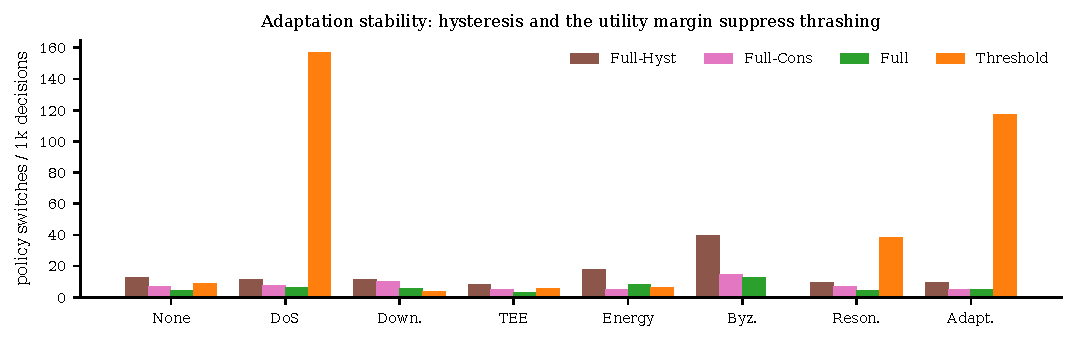
\includegraphics[width=\linewidth]{figures/fig_switching.pdf}
\caption{Policy switches per $1{,}000$ decisions by scenario. Hysteresis and the
utility margin reduce switching by more than half relative to the same controller
without them, including under the adaptive and Byzantine scenarios.}
\label{fig:switching}
\end{figure}

% Generated by make_paper_assets.py — do not edit by hand; regenerate.
\begin{table*}[t]
\centering
\scriptsize
\setlength{\tabcolsep}{3.5pt}
\caption{Policy switches per 1,000 decisions (mean over 10 seeds). A switch is a
change of security level for the same operation class between epochs; the final
column averages the seven attack scenarios. Lower is better; static policies are
omitted because they never switch.}
\label{tab:switching}
\begin{tabular}{lccccccccc}
\toprule
Policy & None & DoS & Down. & TEE & Energy & Byz. & Reson. & Adapt. & Mean \\
\midrule
Threshold & 8.6 & 157.2 & 3.8 & 5.6 & 6.3 & 0.7 & 38.6 & 117.2 & 47.1 \\
Risk-Only & 18.7 & 12.5 & 11.9 & 11.6 & 20.3 & 25.8 & 9.6 & 9.1 & 14.4 \\
Inv.-Only & 0.6 & 6.5 & 0.4 & 0.5 & 0.8 & 0.2 & 4.4 & 0.5 & 1.9 \\
Full$-$Hyst & 12.5 & 11.6 & 11.3 & 8.3 & 18.1 & 39.5 & 9.2 & 9.3 & 15.3 \\
Full$-$Cons & 6.9 & 7.7 & 9.9 & 4.8 & 4.9 & 14.7 & 6.7 & 4.9 & 7.7 \\
\textbf{Full} & 4.3 & 6.1 & 5.9 & 3.4 & 8.2 & 12.5 & 4.5 & 4.8 & 6.5 \\
\emph{Oracle} & 4.1 & 6.4 & 5.6 & 6.1 & 0.0 & 3.1 & 3.2 & 3.2 & 3.9 \\
\bottomrule
\end{tabular}
\end{table*}


\paragraph{Systems cost.} Full's median decision latency is $2.27$\,ms and its
$99$th percentile is $5.54$\,ms, with $0.288$\,mJ per granted decision,
$14$\,KB SRAM and $86$\,KB flash. Static-High is $6.00$\,ms and $0.728$\,mJ with
$4$\,KB and $28$\,KB; Threshold is $1.33$\,ms and $0.295$\,mJ; Invariant-Only is
$1.34$\,ms and $0.239$\,mJ. The full controller is therefore cheaper than a
static-high posture in latency (by a factor of $2.6$) and energy (by a factor of
$2.5$), because it selects the cheapest admissible action most of the time and
pays for deep inspection only when the belief or I3 requires it. It is more
expensive than Invariant-Only by $0.049$\,mJ and $28$\,KB of flash, which is the
cost of the belief filter and trust weights.

These are analytical model outputs, not silicon measurements. The per-layer
constants come from datasheet-level operation counts and the tier mix of
\cref{sec:system-model}; the reported p50/p99 are therefore best read as
relative comparisons between postures, not as predictions for a specific board.
The footprint numbers are model estimates for the static image of the decision
layer and exclude the cryptographic library, which would be shared with any
baseline. A deployment would replace the cost model with a measured profile; the
controller only consumes the resulting scalar costs, so the decision logic does
not change.

% Generated by make_paper_assets.py — do not edit by hand; regenerate.
\begin{table}[t]
\centering
\small
\caption{Systems cost per granted decision, averaged over all 70 runs.
Latency and energy are \emph{analytical model} outputs from datasheet-level
operation costs and the tier mix; SRAM/flash are model footprints, not
silicon measurements.}
\label{tab:systems}
\begin{tabular}{lccccc}
\toprule
Policy & p50 (ms) & p99 (ms) & Energy (mJ) & SRAM (KB) & Flash (KB) \\
\midrule
Static-High & 6.00 & 6.00 & 0.728 & 4.0 & 28.0 \\
Static-Med & 3.40 & 4.70 & 0.472 & 14.0 & 86.0 \\
Static-Low & 0.90 & 0.90 & 0.047 & 4.0 & 28.0 \\
Threshold & 1.33 & 5.17 & 0.295 & 6.0 & 34.0 \\
Risk-Only & 0.90 & 4.74 & 0.113 & 12.0 & 74.0 \\
Inv.-Only & 1.34 & 5.00 & 0.239 & 9.0 & 58.0 \\
Full$-$Hyst & 1.51 & 5.54 & 0.243 & 14.0 & 86.0 \\
Full$-$Cons & 2.40 & 5.60 & 0.294 & 12.0 & 74.0 \\
\textbf{Full} & 2.27 & 5.54 & 0.288 & 14.0 & 86.0 \\
\emph{Oracle} & 2.23 & 5.59 & 0.281 & 14.0 & 86.0 \\
\bottomrule
\end{tabular}
\end{table}


\paragraph{Ablation.} \Cref{tab:ablation} summarises the component analysis over
the seven attack scenarios. Full has the lowest malicious-grant rate ($0.177$) of
the four ablated variants and utility within $0.001$ of Full$-$Hyst; among all
policies that enforce the floor, only Static-High and Oracle have lower exposure
($0.127$ and $0.148$), at lower utility and as an oracle upper bound,
respectively. Removing hysteresis raises malicious grants to $0.209$ and
switches to $15.3$; removing consistency weighting raises malicious grants to
$0.184$ and the energy-scenario Brier score to $0.455$; removing the belief
entirely (Invariant-Only) gives $0.312$ and Brier $0.296$. The order is consistent: the invariant layer carries
safety, the belief and trust weighting carry detection, and hysteresis carries
stability. No single component is responsible for all three.

% Generated by make_paper_assets.py — do not edit by hand; regenerate.
\begin{table}[t]
\centering
\small
\caption{Component ablation (Full policy), means over the seven attack scenarios.
Brier$_{\text{energy}}$ isolates the attack-inflation scenario, where uniform
modality fusion is misled. Switches are per 1,000 decisions.}
\label{tab:ablation}
\resizebox{\textwidth}{!}{%
\begin{tabular}{lcccccc}
\toprule
Variant & IVR/1k & Malicious grant & Utility & Brier$_{\text{energy}}$ & Switches/1k & Energy (mJ) \\
\midrule
Inv.-Only & 0.00 & 0.312 & 0.102 & 0.296 & 1.9 & 0.239 \\
Full$-$Hyst & 0.00 & 0.209 & 0.119 & 0.003 & 15.3 & 0.243 \\
Full$-$Cons & 0.00 & 0.184 & 0.118 & 0.455 & 7.7 & 0.294 \\
\textbf{Full} & 0.00 & 0.177 & 0.120 & 0.003 & 6.5 & 0.288 \\
\emph{Oracle} & 0.00 & 0.148 & 0.128 & 0.000 & 3.9 & 0.281 \\
\bottomrule
\end{tabular}}
\end{table}


\subsection{Sensitivity of the actuation floor}
\label{sec:rq5-floor}

The guarantee in RQ1 is only as strong as the floor it enforces, so we repeat
the Full experiment with four I1 variants: mutual authentication with header
inspection (the default), attestation with header inspection, mutual
authentication with deep inspection, and attestation with deep inspection.
\Cref{tab:floor} reports the result. Every variant keeps IVR at zero, which is
the expected consequence of enforcing the floor; the differences are in residual
exposure, utility and energy. Strengthening I1 from mutual authentication with
header inspection to attestation with deep inspection reduces malicious grants
from $0.177$ to $0.165$ (about $7\,\%$), lowers attack-scenario utility only
from $0.120$ to $0.115$, and raises modelled energy from $0.279$ to
$0.363$\,mJ (about $30\,\%$). Every variant keeps IVR at zero. The two
intermediate floors are not strictly ordered---attestation with header inspection
gives $0.170$ and mutual authentication with deep inspection gives $0.171$---which
is within seed noise and illustrates that the components buy different, partly
substitutable evidence rather than a single strength scale.

This sensitivity is the practical answer to the \texttt{tee} result. Since the
belief cannot be trusted when the anchor is subverted, the defensible response is
to choose the floor using an explicit risk budget rather than to tune the
estimator until it looks better on the out-of-model scenario. \Cref{tab:floor}
makes that choice legible.

% Generated by floor_sensitivity.py — do not edit by hand; regenerate.
\begin{table}[t]
\centering
\caption{Sensitivity to the actuation floor (I1), Full policy, 10 seeds.
IVR, false denial and energy are means over all eight scenarios; malicious
grant and utility (marked $^{\ast}$) are means over the seven attack scenarios.
Every floor keeps invariant violations at zero; a stronger floor buys lower
residual exposure at a utility and energy cost.}
\label{tab:floor}
\resizebox{\textwidth}{!}{%
\begin{tabular}{lccccc}
\toprule
Actuation floor & IVR/1k & Malicious grant$^{\ast}$ & Utility$^{\ast}$ & False deny & Energy (mJ) \\
\midrule
mutual auth + header IDS & 0.00 & 0.177 & 0.120 & 0.026 & 0.279 \\
attestation + header IDS & 0.00 & 0.170 & 0.118 & 0.028 & 0.288 \\
mutual auth + deep IDS & 0.00 & 0.171 & 0.117 & 0.029 & 0.357 \\
attestation + deep IDS & 0.00 & 0.165 & 0.115 & 0.030 & 0.363 \\
\bottomrule
\end{tabular}}
\end{table}


\subsection{Trace-derived calibration}
\label{sec:trace}

The simulator's network-intensity prior is calibrated against the public IoT-23
capture \cite{garcia2020iot}. We extract individual \texttt{conn.log.labeled}
captures, aggregate packet counts into $60$\,s bins, separate benign from
malicious bins using the capture labels, and fit a log-normal rate model. The
contrast is the difference of mean log rates, estimated only within captures that
contain both labels so that a device/context difference between captures cannot
masquerade as an attack effect. The fitted benign mean log-rate is $-3.103$ and
the malicious mean is $-1.413$, giving a contrast of $1.689$ with a
$2{,}000$-sample stratified bin bootstrap interval of $[1.652,1.726]$
(\cref{tab:trace}). The two within-capture estimates are $1.131$ and $2.570$;
that spread, not the bin-level interval, is the honest between-capture
uncertainty, and the bin bootstrap understates it because consecutive bins are
autocorrelated. The simulator uses a benign mean of $4.20$ and a DoS mean of
$5.889$, a contrast of $1.689$. The absolute rates differ because a sparse
honeypot capture is not comparable to per-node application telemetry, so only the
contrast is matched. The dispersion is not matched either: the simulator's
network standard deviation is $0.50$ benign and $0.55$ under DoS, against pooled
log-rate standard deviations of $0.65$ and $0.86$ in the trace, so no
distributional-shape claim is made.

\Cref{fig:belief-trace} shows the belief, the minimum modality trust and the
consistency score on one adaptive-attack run. The belief rises inside the attack
windows and decays after them; the trust on the network modality falls when the
spoofed context diverges from the device anchor and recovers slowly; the
consistency score leads the belief during the early part of an attack. The
figure is a single seed and is included as an illustration of the mechanism, not
as evidence of average performance; the aggregate numbers are in
\cref{tab:calibration,tab:detection}.

\begin{figure}[t]
\centering
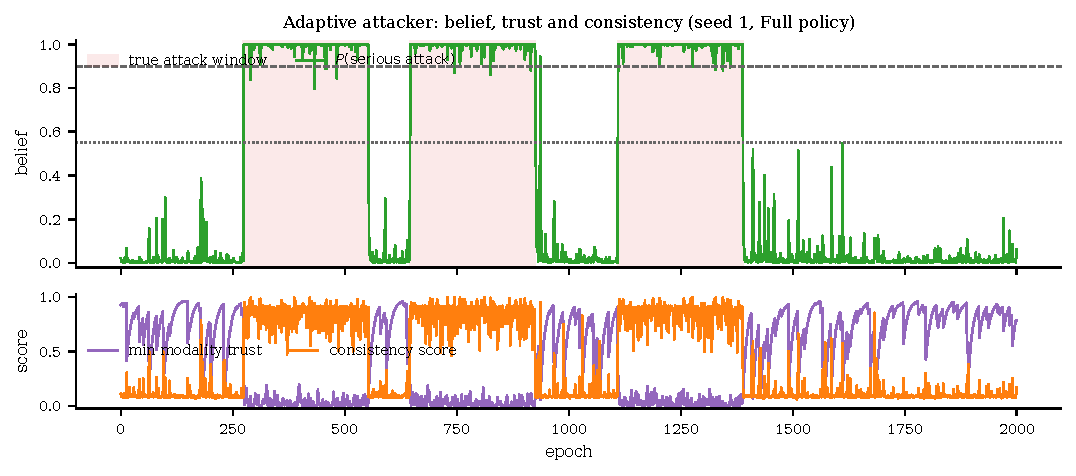
\includegraphics[width=\linewidth]{figures/fig_belief_trace.pdf}
\caption{Belief, minimum modality trust and consistency score on one adaptive
attack run (seed 1, Full policy). The belief rises in the attack windows and
decays afterwards; distrust is fast and restoration is slow. Single-seed
illustration, not an aggregate result.}
\label{fig:belief-trace}
\end{figure}

\begin{figure}[t]
\centering
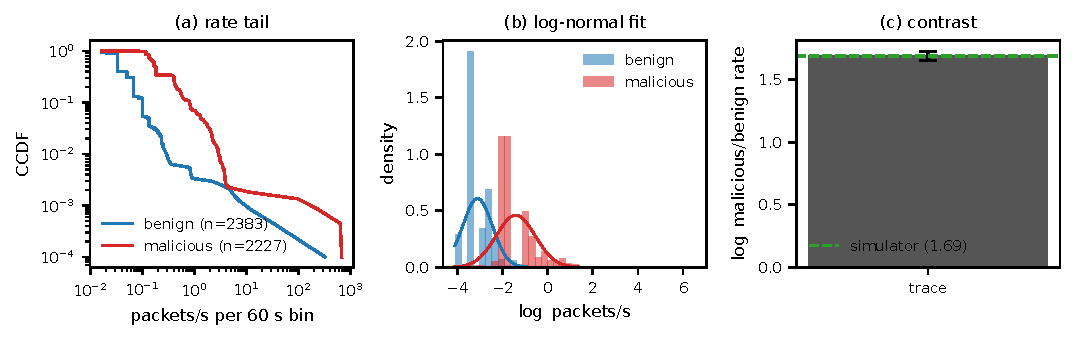
\includegraphics[width=\linewidth]{figures/fig_trace_calibration.pdf}
\caption{IoT-23 calibration of the network-intensity prior. Benign and malicious
$60$\,s bins are separated by capture label; the fitted mean-log-rate contrast is
$1.689$ with per-capture values $1.131$ and $2.570$. The simulator matches the
contrast, not the absolute rate or the dispersion.}
\label{fig:trace}
\end{figure}

% Generated by make_paper_assets.py from trace_priors.json.
\begin{table}[t]
\centering
\small
\caption{IoT-23 trace calibration of the network-intensity prior. The contrast is
the difference of mean $\log$ rates over 60\,s bins, estimated only within
captures that contain both benign and malicious traffic. The bracket is a
2{,}000-sample stratified bin bootstrap, which treats bins as independent; the
per-capture values show the between-capture spread. Absolute rates are not
comparable to per-node simulator telemetry; only the contrast is calibrated.}
\label{tab:trace}
\begin{tabular}{lcc}
\toprule
Quantity & Trace & Simulator \\
\midrule
Benign 60\,s bins & 2383 & -- \\
Malicious 60\,s bins & 2227 & -- \\
Benign $\log$ rate (mean) & -3.103 & 4.20 \\
Malicious $\log$ rate (mean) & -1.413 & 5.89 \\
Log-rate contrast & 1.689 [1.652, 1.726] & 1.689 \\
\quad per-capture contrast & 1.131, 2.570 & -- \\
\bottomrule
\end{tabular}
\end{table}


\subsection{Summary of the evidence}
\label{sec:eval-summary}

The five research questions receive the following answers. RQ1: yes, with a
zero IVR in every scenario, and the zero is structural rather than a property of
the estimator (\cref{tab:ivr,tab:ivr-byop}). RQ2: the guarantee costs little
utility relative to Static-High ($+0.036$) and gains more against Threshold
($+0.043$), it cuts false denials by a factor of three, but it grants more
malicious requests than Static-High ($0.177$ versus $0.127$), mostly in the
out-of-model TEE scenario, because the invariant floor bounds the action, not the
adversary's credential (\cref{tab:utility,tab:falsedeny,tab:exposure}). RQ3: the
belief is well calibrated under DoS, in-model downgrade, energy inflation,
resonant, Byzantine and adaptive attacks, and fails only when the attestation
anchor is subverted; trust weighting is worth a factor of about $140$ in Brier score
under energy inflation (\cref{tab:calibration,tab:detection}). RQ4: the
per-operation envelope denies $0.029$ of safety requests against $0.088$ for
Static-High, and every residual denial is a mechanism false positive, not a
policy choice (\cref{tab:safety}). RQ5: switching is $6.5$ per $1{,}000$
decisions against $15.3$ without hysteresis, and the full controller is cheaper
than Static-High in latency ($2.27$ versus $6.00$\,ms) and energy ($0.288$ versus
$0.728$\,mJ) at the cost of $28$\,KB of flash relative to Invariant-Only
(\cref{tab:switching,tab:systems}). Strengthening the actuation floor reduces
exposure without changing IVR (\cref{tab:floor}). The next section discusses what
these results do and do not establish.

\section{Discussion}
\label{sec:discussion}

\subsection{What the results establish}
\label{sec:what-established}

The central claim of the paper is an architectural separation: adaptation may
choose among safe actions, but it may not choose whether an action is safe. The
experiments support that separation in a specific and limited sense. The
invariant-violation rate is zero for every policy that enforces I1/I2, and it
remains zero in the scenario where the belief is demonstrably wrong. This is not
because the estimator is good; it is because the estimator has no authority over
the floor. The Risk-Only ablation makes the counterfactual concrete: the same
trust-weighted Bayesian machinery without the floor violates the floor at $327.41$
per $1{,}000$ decisions, close to the $393.31$ of a policy that ignores risk
entirely. The node-side PEP re-check is what closes the gap between a gateway
decision and an enforced action.

The utility result is positive but modest, and should be read carefully. Full
attains $0.120$ mean attack-scenario utility against $0.084$ for Static-High and
$0.077$ for Threshold, a paired gain of $+0.036$ and $+0.043$
($p_{\text{Holm}}=0.008$ in both cases). It also cuts the false-denial rate from
$0.088$ to $0.027$. Those are real effects on a normalised scale, but they are
smaller than the differences against policies that are either unsafe (Static-Low,
Risk-Only) or over-deny. A reader who expects a context-adaptive controller to
dominate a static-high posture on every metric will not find that here, and the
paper does not claim it: Static-High still has lower residual exposure
($0.127$ versus $0.177$).

The belief result is conditional, and the condition is now explicit. Trust-weighted
fusion is valuable when the adversary poisons a subset of modalities: the Brier
score under energy inflation improves from $0.455$ for uniform fusion to $0.003$
for Full. It is also sufficient for the in-model downgrade, where the attested
device anchor and the cross-node dispersion survive the spoof: the belief AUROC is
$1.000$ and the Brier score is $0.003$. It is not sufficient when the adversary
also controls the attestation anchor. In the \texttt{tee} scenario the Brier score
is $0.437$, the poisoning AUROC is $0.273$ (below chance) and the malicious-grant
rate rises to $0.473$. That negative result is the strongest argument for the
architecture, because a design that relied on detection would fail exactly where
this one remains safe.

\subsection{Limitations}
\label{sec:limitations}

\paragraph{Simulation, not deployment.} All performance numbers come from a
parameterised discrete-time simulator. The observation model, transition matrix
and attack processes are explicit and the streams are paired, but they are not a
real deployment. Latency, energy and footprint are analytical estimates from
datasheet-level operation costs, not measurements on the three hardware classes.
The relative comparison between postures is meaningful; the absolute numbers are
not predictions for a specific board. A hardware testbed is the obvious next
step.

\paragraph{A subverted anchor is not solved.} The paper does not claim that the
belief detects a compromise of the node's trusted execution environment. On the
contrary, \cref{tab:detection} shows that both the poisoning AUROC ($0.273$) and
the belief AUROC ($0.210$) are below chance in the \texttt{tee} scenario, and
\cref{tab:utility} shows that Full's attack-scenario utility drops to $0.058$
there---far below its usual level, even though it edges Static-High ($0.053$)
because both postures become cheap. The guarantee survives because I1/I2 are
unconditional, but the posture selected inside the envelope can still be too
cheap, which is why residual malicious grants rise to $0.473$. Closing that gap requires evidence the
adversary cannot fabricate---hardware attestation rooted outside the TEE, physical
invariants, or out-of-band confirmation---not a better classifier on the same
features. The in-model downgrade, by contrast, is handled: the belief stays
calibrated because the anchor and dispersion are retained.

\paragraph{The floor bounds the action, not the credential.} A malicious request
that holds a valid credential and arrives with a plausible context can be granted
an action that satisfies I1. The invariant layer ensures that such an action uses
strong authentication, AEAD, freshness and inspection; it does not ensure that the
request is benign. This is why Full's malicious-grant rate ($0.177$) is higher than
Static-High's ($0.127$). Most of the gap is the out-of-model \texttt{tee} scenario:
excluding it, Full is $0.128$ against $0.104$. The floor is a bound on the
\emph{mechanism}, not on the \emph{authorisation decision}. Reducing residual
exposure requires either a stronger unconditional floor
(\cref{sec:rq5-floor}) or an authorisation layer that is outside the scope of this
paper.

\paragraph{Trust anchors.} The device modality is treated as an attestation
anchor. If a node's trusted execution environment is subverted, the anchor is no
longer trustworthy and the trust weighting can be steered by the compromised node;
this is the \texttt{tee} scenario, deliberately reported rather than hidden. I1
still limits what that node can do to other physical processes, but it cannot
prevent the node from exercising credentials it legitimately holds. The same caveat
applies to a compromised gateway: the PDP is trusted in this model, and a gateway
compromise is out of scope.

\paragraph{Model and tuning.} The emission model, transition matrix and cost
weights are the defender's assumptions. In this simulator the likelihood is
evaluated with the same parameters that generate the observations, so the belief
is correctly specified by construction and the calibration and detection results
are an oracle-model upper bound; a defender with a misspecified model would do
worse. The thresholds in \cref{tab:params} were fixed before the final ten-seed
matrix was generated, but
they were selected using earlier runs on the same simulator; this leaves a risk of
optimistic bias that a pre-registered, held-out parameter search would remove. The
violation penalty $\rho=6.0$ is a reporting convention, not a controller
parameter; because the proposed controller never grants a below-floor action, its
utility is unaffected by $\rho$, while the unconstrained baselines are penalised
for violations they actually commit. The floor sensitivity (\cref{tab:floor}) and
the component ablation (\cref{tab:ablation}) are included partly to make the
dependence on those choices visible. The action lattice is finite ($243$ actions),
the deployment is $24$ nodes, and the Byzantine fraction is $10/24$; larger or
heterogeneous deployments may shift the quantitative trade-offs even if the
structural argument is unchanged.

\paragraph{Baselines.} The baselines are deliberately simple. Threshold is a
univariate point estimate on the same anomaly feature the adversary manipulates;
we raise it to the structural floor so that its IVR is not an artefact, but we do
not evaluate a multivariate or learned detector tuned to Full's false-positive
rate. Static-Med is a fixed mid-point and Static-High is the strongest uniform
posture. A learned detector could close part of the utility gap without the
belief, and a detector trained on the simulator's oracle-model features would look
better than one trained on real telemetry. The comparison therefore isolates the
architecture---belief, floor and PEP---rather than the best achievable detector.

\paragraph{Trace calibration is partial.} The IoT-23 capture is a honeypot
dataset; its absolute rates are not comparable to per-node application telemetry,
and we match only the benign-to-malicious mean-log-rate contrast ($1.689$, with
per-capture values $1.131$ and $2.570$). The simulator's network dispersion is
narrower than the trace ($0.50$ and $0.55$ versus $0.65$ and $0.86$), so no
distributional-shape claim is made. The capture does not exercise the controller,
the request process or the physical process, so it cannot validate the utility or
safety results. It constrains one prior, and we describe it as such.

\paragraph{Adversary strength.} The attacker is white-box but not an optimal
POMDP solver. The adaptive scenario increases the spoofed fraction over time and
then holds the anomaly just below the public point-estimate threshold, and the
resonant scenario pulses near the dwell period, but neither is a worst-case policy
computed against the defender's model. A stronger adversary could search for
belief trajectories that keep the controller at the cheapest admissible action for
longer; the floor would still hold, but the utility and exposure numbers would move
against the defender.

\subsection{Threats to validity}
\label{sec:validity}

\paragraph{Construct validity.} Mission utility is a weighted sum of value,
damage, denial cost, energy and latency, and it is reported after subtracting a
violation penalty $\rho$ for any granted action below the floor. The weights are
design choices, and a different operator could rank postures differently. We
mitigate this by reporting the components separately (utility, false denial,
malicious grant, safety denial) rather than only the composite, and by showing the
floor sensitivity. The IVR, false-denial and safety-denial metrics are direct
counts and do not depend on the utility weights or on $\rho$.

\paragraph{Internal validity.} All policies within a seed and scenario replay the
same observation and request stream, which removes stream-to-stream variance from
the comparison. The simulator is deterministic given the seed, and the unit tests
check the invariant mask, the belief normalisation, the trust bounds, the
fail-safe fallback and the paired-stream property. The main internal threat is
parameter tuning on the same scenario family, discussed above. A second threat is
that the stochastic detection model is shared by all policies, so a policy cannot
gain by exploiting a different mechanism model; this is intentional for
comparability but means the absolute detection rates are model artefacts.

\paragraph{External validity.} The results are for a 24-node deployment with three
hardware classes, one action lattice and eight scenarios. The qualitative
claim---a hard floor decouples safety from estimation error---is not specific to
these numbers, but the magnitude of the utility and exposure trade-offs is. The
IoT-23 calibration improves the realism of one prior without making the simulator a
trace replay.

\paragraph{Conclusion validity.} The paired tests use ten seeds and a conservative
non-parametric test, with each seed's seven attack scenarios aggregated into one
mean before testing. That aggregation is a deliberate summary, not seven
independent scenario tests: with ten pairs the smallest attainable two-sided
$p$-value is $0.00195$, so every $p_{\text{Holm}}=0.008$ in \cref{tab:stats} sits
at the resolution floor and should be read as sign consistency across seeds, not
as a precise significance level. We therefore lead with effect sizes and the
per-scenario breakdown, and we do not claim scenario-specific significance. The utility
difference against Static-High ($+0.036$) is small but reliably positive
($p_{\text{Holm}}=0.008$); the exposure difference ($+0.050$) is larger and goes
against the proposed policy. Both are reported.

\subsection{Design implications}
\label{sec:implications}

Three implications follow for practitioners. First, the safety floor should be
chosen as an explicit risk budget, not as a by-product of estimator tuning. The
floor sensitivity in \cref{tab:floor} shows how strengthening I1 trades exposure
against utility and energy; an operator can pick a point on that curve without
changing the controller. Second, the attestation anchor is load-bearing: if the
device modality is not rooted in hardware the adversary cannot rewrite, the
downgrade failure becomes easier to induce. Third, the PDP/PEP split matters: the
belief and the scorer can run on a gateway, but the admissible-set check and the
fail-safe action must run on the node, or a network adversary can bypass them.

\subsection{Ethics and reproducibility}
\label{sec:ethics}

The work uses a public network capture and a simulator; it involves no human
subjects and no private data. The attack scenarios are defensive stress tests, and
the paper does not release an exploit. The dual-use risk is the usual one for
access-control research: a description of how context poisoning defeats a CAAC
policy could be misused. We judge the defensive value to outweigh that risk, and
the design specifically aims to make the attack less effective by removing the
estimator's authority over the safety floor.

The simulator, the analysis scripts and the generated tables are deterministic
given the seeds and are organised so that every reported number can be regenerated
from the frozen matrix. The manuscript does not contain hand-typed experimental
values; the asset generator reads the CSV and writes both the tables and the prose
summary used for cross-checking.

\section{Related Work}
\label{sec:related}

\subsection{Access control models and context adaptation}

Access control has a long line of models that separate policy from mechanism.
Role-based access control assigns permissions to roles \cite{sandhu1996role};
attribute-based access control generalises the decision to subject, resource and
environment attributes \cite{hu2014guide}; usage control adds continuity and
revocation during use \cite{park2004ucon}. These models provide the vocabulary
for \emph{what} is permitted, but they leave the strength of the enforcing
mechanism to configuration. Zero-trust architectures make the mechanism
explicitly dynamic and assume no implicit trust from network location
\cite{rose2020zero,federici2023zero,zanasi2024flexible,stodt2025beyond}; our work
shares the ``never trust the context unconditionally'' premise but focuses on
the safety of the resulting action rather than on identity verification alone.

Context-adaptive access control (CAAC) makes the posture a function of device
and environmental context \cite{atlam2017overview,rath2017adaptive,genc2019context,arfaoui2019context}.
Recent designs add blockchain-backed continuous authentication
\cite{hussainalnaji2022cab}, smart-contract policy evaluation
\cite{merlec2024sc}, role--capability combinations \cite{krishnasrija2025dynamic},
and app-independent policy enforcement for IoT platforms \cite{mazhar2023maverick}.
Surveys document the breadth of the area and the recurring use of a point risk
estimate as the interface between monitoring and enforcement
\cite{ravidas2019access,qiu2020survey,elhajj2019survey}. Learning-based access
control \cite{nobi2022deep} and context-aware computing more generally
\cite{piccialli2021context} push in the same direction: richer context, more
adaptive decisions. What is usually missing is an explicit adversary who controls
the context channel and an explicit statement of which parts of the decision are
not tradeable. Our contribution is not a new access-control model but a
constrained formulation in which the adaptation is confined by construction to an
already-safe set.

\subsection{Risk estimation and uncertainty}

Risk-based access control uses a score to choose among authentication factors
\cite{lee2017situational,moura2017sotraace}. The score is typically a point
estimate, sometimes with a threshold and sometimes with a cost model. Our belief
is a forward hidden Markov model \cite{rabiner1989tutorial} over latent threat
states, which is a standard partially observable formulation
\cite{kaelbling1998planning}; the difference is that we evaluate it with proper
scoring rules \cite{gneiting2007strictly} and calibration error
\cite{guo2017calibration}, and we do not let it override the invariants.
Self-explainable cyber-physical systems \cite{blumreiter2019self} and
dependability taxonomies \cite{avizienis2004basic} provide complementary
vocabularies for reasoning about why a decision was taken and how it can fail;
we use the latter implicitly in the per-operation failure semantics.

\subsection{Runtime assurance and safety shields}

The closest architectural relatives are runtime assurance and shield synthesis.
The Simplex architecture keeps a verified baseline controller and switches to it
when the advanced controller is untrusted \cite{sha2001simplicity}; safety guards
and shield synthesis enforce a temporal property at the actuator boundary
\cite{wu2017safety,wu2019shield}; the black-box Simplex architecture extends the
idea to learned components \cite{mehmood2022black}; and recent work generates
verified monitors from timed automata \cite{cho2025timed}. Our admissible-set
constructor plays the role of the baseline, and the I4 fallback plays the role of
the switch. The difference is the plant: the actions are access-control postures
in a $243$-element lattice rather than a scalar control input, and the safety
property is a per-operation envelope over authentication, cryptography,
inspection, rate limiting and freshness. The invariant-dominance and
structural-safety propositions are the analogue of the Simplex safety argument
for this lattice. A Simplex-style baseline here would hold a fixed strong posture
as the verified fallback and switch to the adaptive posture only when a monitor
certifies the context; without such a certificate it reduces to Static-High,
which is exactly the low-utility, high-false-denial point in our results. We do
not implement that baseline because the certificate would be the same belief we
are testing, so it would not provide an independent control.

\subsection{Poisoning, Byzantine context and denial of sleep}

Sensor spoofing and false data injection are well studied in cyber-physical
systems \cite{barua2020special,li2019optimal}, and consistency checks can detect
attacks that violate physical invariants \cite{ye2020summation}. Byzantine fault
tolerance bounds the influence of faulty nodes when fewer than half collude
\cite{lamport1982byzantine}, and resilient architectures apply the bound to
industrial and aviation systems \cite{alsulami2021resilient}. Our Byzantine
scenario uses the same $f<N/2$ assumption and adds a cross-node dispersion
signal, but the bound is used only to keep the aggregate informative; it does not
by itself make the interpretation correct. Denial-of-sleep attacks exploit the
reverse incentive, forcing a device to spend energy on security work
\cite{brownfield2005wireless,raymond2009effects}. The energy-inflation and
resonant scenarios are direct stress tests of that failure mode, and the
asymmetric trust update is designed so that a false alarm is corrected slowly, not
immediately amplified.

\subsection{Datasets, calibration and lightweight enforcement}

Public IoT intrusion datasets include IoT-23 \cite{garcia2020iot}, Edge-IIoTset
\cite{ferrag2022edge}, CICIoT2023 \cite{neto2023ciciot2023}, BoT-IoT
\cite{koroniotis2019development}, ToN-IoT \cite{moustafa2020data} and NetFlow-based
evaluation platforms \cite{moustafa2021new}; transformer-based detectors are
commonly evaluated on them \cite{tseng2024multi}. These datasets support
signature and anomaly detection, not access-control decisions under an adaptive
context adversary, which is why we use one of them only to calibrate a prior and
generate the rest of the evaluation from an explicit model. At the enforcement
layer, Ascon is standardised for constrained devices
\cite{dobraunig2021ascon}, and implementation studies report microcontroller
costs \cite{cagua2025implementation}. We treat the cryptographic primitives as
correct and model their cost; the contribution is the decision layer that
selects among them.

\subsection{Positioning}

\Cref{tab:positioning} summarises the distinction. Existing CAAC work optimises
an expected objective against a point estimate and has no non-negotiable floor;
runtime assurance enforces a floor but for a scalar control input rather than an
access-control lattice; Byzantine and poisoning work characterises what an
adversary can do to an aggregate but not what the enforcement point should do
when the aggregate is wrong. This paper combines the three: a constrained CAAC
formulation, an explicit per-operation fail-safe semantics, and an evaluation
that includes the case where the belief is successfully fooled.

\begin{table}[t]
\centering
\small
\caption{Positioning against the three closest lines of work.}
\label{tab:positioning}
\begin{tabular}{p{0.22\linewidth}p{0.30\linewidth}p{0.30\linewidth}}
\toprule
Line of work & What it provides & What it leaves open \\
\midrule
CAAC / risk-based AC
& Context-dependent posture, point risk score
& No non-negotiable floor; estimator error becomes policy error \\
Runtime assurance / shields
& Verified baseline, switching argument
& Scalar control input, not an access-control action lattice \\
Byzantine / poisoning
& Bounds on aggregate influence, attack detectability
& What the enforcement point does when the aggregate is wrong \\
\textbf{This paper}
& Constrained CAAC with I1--I4, per-operation fail-safe action
& Hardware validation, optimal adversary, credential misuse \\
\bottomrule
\end{tabular}
\end{table}

\section{Conclusion}
\label{sec:conclusion}

Context-adaptive access control is useful precisely because it can lower its
guard, and that is also why it is dangerous. This paper argued that the
adaptation should be confined to a set that is already safe. We formalised a
constrained control problem over five latent threat states, four context
modalities and a $243$-element action lattice, with four invariants: an
unconditional actuation envelope (I1), an unconditional safety-traffic envelope
(I2), a belief-conditional restriction that can only narrow the set (I3), and
per-operation failure semantics that fail closed for confidentiality and
integrity operations and fail-safe-allow for certified safety operations (I4).
A forward Bayesian belief with cross-modal trust weights and a cross-node
dispersion signal chooses among the admissible actions; it has no authority over
the set itself.

The evaluation supports the separation. Across $800$ runs, every
invariant-enforcing policy records zero invariant violations per $1{,}000$
decisions, including in the \texttt{tee} scenario where the belief is confidently
wrong; the unconstrained risk-adaptive policy records $327.41$ and the static-low
policy $393.31$. The full controller reaches $0.120$ mean attack-scenario utility
against $0.084$ for static-high and $0.077$ for threshold CAAC, and denies
$0.029$ of safety-critical requests against $0.088$ for static-high. It is
cheaper than static-high in decision latency ($2.27$\,ms versus $6.00$\,ms) and
modelled energy ($0.288$\,mJ versus $0.728$\,mJ), and it reduces policy switching
from $15.3$ to $6.5$ per $1{,}000$ decisions relative to the same controller
without hysteresis.

The honest negative result is residual exposure. The invariant floor bounds the
mechanism of a granted action, not the credential of the requester: the full
controller grants $0.177$ of malicious requests against $0.127$ for static-high,
and the gap is concentrated in the out-of-model case where the node's trusted
execution environment is subverted ($0.473$ malicious grants, Brier $0.437$,
poisoning AUROC $0.273$). Within the stated threat model, the attested device
anchor and cross-node dispersion survive poisoning: the in-model downgrade yields
a Brier score of $0.003$ and a belief AUROC of $1.000$. Strengthening the
actuation floor to attestation plus deep inspection reduces malicious grants
without changing the zero-violation result, which is the right way to buy
exposure down once the estimator has been shown to be spoofable. The guarantee is
carried by the unconditional invariants; the belief improves utility and detection
when it can, and its failure does not become a safety failure.

Several directions remain. The most important is a hardware testbed that replaces
the analytical cost model with measured latency and energy on the three tiers. A
second is a stronger adversary that computes a policy against the defender's model
rather than following the scripted adaptive and resonant patterns; the invariant
argument would survive, but the utility and exposure numbers would be a better
bound. A third is out-of-band evidence---physical invariants, attestation rooted
outside the node TEE, or independent channels---that a full-modality spoof cannot
fabricate, which is the only way to close the \texttt{tee} gap rather than merely
bound its damage. Finally, the admissible-set constructor and the fail-safe
fallback are small enough to be verified with the timed-automata and
monitor-generation techniques that runtime assurance has developed, and doing so
would turn the structural argument of \cref{prop:structural} into a machine-checked
property of the implementation.

\section*{Data and code availability}

The simulator, the analysis scripts, the frozen $800$-run matrix and a
one-command reproduction procedure are available at
\url{https://github.com/DrMahmoudAljawarneh/failsafe-caci-iot}. The IoT-23 capture
used for the prior calibration is publicly available from the Stratosphere
Laboratory \cite{garcia2020iot}.


\bibliographystyle{elsarticle-num}
\bibliography{references}

\end{document}
